\synctex=1
\documentclass[a4paper,11pt,svgnames]{book}

\usepackage[utf8x]{inputenc}
\usepackage{mathtools}
\usepackage{thesis}
\usepackage{calc}
\usepackage{enumitem}
\setlength{\marginparwidth}{2cm}
\setlength{\voffset}{-0.25in}
\setlength{\parskip}{0.1in}

%\includeonly{5-architecture}
%\includeonly{6-use-case}

%\usepackage{draftwatermark}
%\SetWatermarkScale{4}
\usepackage{subfig}
 \usepackage{listings}
  \usepackage{courier}
 \lstset{
 	 basicstyle=\footnotesize\ttfamily,
         numbers=none,               
         numberstyle=\tiny,          
         %stepnumber=2,              
         numbersep=5pt,              
         tabsize=2,
         extendedchars=true,         
         breaklines=true,            
         keywordstyle=\color{red},
      	 frame=single,         
         stringstyle=\color{white}\ttfamily, 
         showspaces=false,           
         showtabs=false,             
         belowcaptionskip=5pt, 
         xleftmargin=2em, 
         xrightmargin=0.8em,
         showstringspaces=false 
 }
 \lstloadlanguages{% Check Dokumentation for further languages ...
         Python,
         Java
 }

\usepackage{caption}

\DeclareCaptionFont{white}{\color{white}}
\DeclareCaptionFormat{listing}{\colorbox{gray}{\parbox{\textwidth-20pt}{#1#2#3}}\vspace{0.01cm}}
\captionsetup[lstlisting]{format=listing,labelfont=white,textfont=white}

\captionsetup[lstlisting]{format=listing,labelfont=white,textfont=white, singlelinecheck=false, margin=0pt, font={bf,footnotesize}}


\usepackage{url}
\usepackage{tabularx}
\usepackage{graphicx}
\usepackage[usenames,dvipsnames,table]{xcolor}
\usepackage{verbatim}
\usepackage[section]{placeins}
\usepackage{hhline}
\usepackage{multirow}

% Define the acronyms
\usepackage{acronym}

%acronym
\acrodef{BDI}{Belief Desire Intention}
\acrodef{BB}{Belief Base}
\acrodef{BML}{Behavior Markup Language}
\acrodef{ECA}{Embodied Conversational Agents}
\acrodef{IE}{Information Extraction}
\acrodef{ITS}{Intelligent Tutoring System}
\acrodef{IR}{Information Retrieval}
\acrodef{JLOO}{Java Learning Objects Ontology}
\acrodef{KB}{Knowledge-Base}
\acrodef{LOD}{Linked Open Data}
\acrodef{NL}{Natural Language}
\acrodef{NLI}{Natural Language Interface}
\acrodef{NLP}{Natural Language Processing}
\acrodef{NLU}{Natural Language Understanding}
\acrodef{MAS}{Multi Agent System}
\acrodef{PoS}{Part of Speech}
\acrodef{QA}{Question Answering}
\acrodef{SKOS}{Simple Knowledge Organization System}
\acrodef{SPARQL}{SPARQL Protocol and RDF Query Language}
\acrodef{SW}{Semantic Web}
\acrodef{OoB}{Out of Band}


\usepackage[pdftex,
            pdfauthor={Alberto Mardomingo Mardomingo},
            pdftitle={Design of a personal agent integrated with a Linked Data Indexing System},
            pdfsubject={Master Thesis},
            pdfkeywords={Semantic, Linked Data, RDF, Scrapping, natural language},
            pdfproducer={PDFTex},
            colorlinks=true,linkcolor=black,citecolor=black,urlcolor=black,hypertexnames=false]{hyperref}

\setcounter{secnumdepth}{3}

\usepackage{framed}

\usepackage{listings}
\lstset{escapeinside=||}

\newcommand\JSONstringvaluestyle{\color{red}}

% switch used as state variable
\newif\ifcolonfoundonthisline

\lstdefinelanguage{JavaScript}{
  keywords={typeof, new, true, false, catch, function, return, null, catch, switch, var, if, in, while, do, else, case, break},
  keywordstyle=\color{blue}\bfseries,
  ndkeywords={class, export, boolean, throw, implements, import, this},
  ndkeywordstyle=\color{darkgray}\bfseries,
  identifierstyle=\color{black},
  sensitive=false,
  comment=[l]{//},
  morecomment=[s]{/*}{*/},
  commentstyle=\color{purple}\ttfamily,
  stringstyle=\color{red}\ttfamily,
  captionpos=b,
  morestring=[b]',
  morestring=[b]"
}


\lstdefinelanguage{json}{
  showstringspaces    = false,
  keywords            = {false,true,q,rows,wt,fl},
  alsoletter          = 0123456789.,
  morestring          = [s]{"}{"},
  stringstyle         = \ifcolonfoundonthisline\JSONstringvaluestyle\fi,
  MoreSelectCharTable =%
    \lst@DefSaveDef{`:}\colon@json{\processColon@json},
  basicstyle          = \ttfamily,
  keywordstyle        = \ttfamily\bfseries,
  captionpos	      = b
}

\definecolor{darkblue}{rgb}{0.0,0.0,0.6}

\lstdefinestyle{listXML}{language=XML, basicstyle=\ttfamily\diny, extendedchars=true,  belowcaptionskip=5pt,xleftmargin=0.4em, xrightmargin=0.3em, numbers=none, frame=single, breaklines=true, breakatwhitespace=true, breakindent=0pt, emph={}, emphstyle=\color{red}, basicstyle=\small\ttfamily, columns=fullflexible, showstringspaces=false, commentstyle=\color{gray}\upshape,
morestring=[b]",
morecomment=[s]{<?}{?>},
morecomment=[s][\color{orange}]{<!--}{-->},
keywordstyle=\color{cyan},
stringstyle=\color{black},
tagstyle=\color{darkblue},
morekeywords={xmlns, version, type, field, copyField, fieldType}
}



\lstdefinestyle{mono}{
   framesep=8px,
   extendedchars=true,
   basicstyle=\ttfamily,
   showstringspaces=false,
   showspaces=false,
   tabsize=2,
   breaklines=true,
   showtabs=false,
   xleftmargin=8pt,
   xrightmargin=8pt
}


\lstdefinestyle{commands}{
   framesep=8px,
   extendedchars=true,
   basicstyle=\ttfamily,
   showstringspaces=false,
   showspaces=false,
   tabsize=2,
   breaklines=true,
   showtabs=false,
   xleftmargin=8pt,
   xrightmargin=8pt
}

\lstdefinestyle{consola}
   {basicstyle=\scriptsize\ttfamily,
    backgroundcolor=\color{white},
    frame=lrtb,
    numbers=none,
    xleftmargin=4pt,
    xrightmargin=4pt
   }


\definecolor{chapterdetails}{HTML}{6DBAFF}

\usepackage[sf,bf]{titlesec}
\titleformat{\chapter}[display]
  {\normalfont\Large\sffamily\raggedleft}
  {\vspace{5cm}\MakeUppercase{\chaptertitlename}%
    \rlap{ \resizebox{!}{1.5cm}{\thechapter} \color{chapterdetails}\rule{5cm}{1.5cm}}}
  {10pt}{\Huge}[{\color{chapterdetails}\titlerule[0.8mm] }]
\titlespacing*{\chapter}{0pt}{30pt}{20pt}

\newenvironment{chapterintro}
{% This is the begin code
\large\it
}
{% This is the end code
}


% Tick symbols
\newcommand{\tickYes}{\checkmark}
\newcommand{\tickNo}{\hspace{1pt}\ding{55}}
% Fancy header
\usepackage{fancyhdr}
%Fancy chapter cover style


% Fancy box
\usepackage{fancybox} 
\setlength{\fboxrule}{1 pt} \setlength{\fboxsep}{10pt} \setlength{\shadowsize}{3pt}

%Sky color definition


\begin{document}
\newcommand\litem[1]{\item{\bfseries #1 }}
\renewcommand{\arraystretch}{1.5} %Makes tables less crammed

\newcommand\headcell[1]{%
  \multicolumn{1}{|c|}{\cellcolor{DodgerBlue}\bfseries\sffamily\textcolor{white}{#1}}
}

\pagenumbering{Roman}

\cleardoublepage
\thispagestyle{empty}
\vspace*{3\baselineskip}
{\large{\bf PROYECTO FIN DE CARRERA}}
\vspace{0.5cm}

\begin{rm}
\begin{tabular}{p{3cm}p{10cm}}
\textbf{Título:} & Desarrollo de un Asistente Personal integrado con un Sistema de Indexación Semántica de Información\\ 
\textbf{Título (inglés):} & Design of a personal agent integrated with a Linked Data System\\ 
\textbf{Autor:} & Alberto Mardomingo Mardomingo \\ 
\textbf{Tutor:} & Carlos A. Iglesias Fernández\\ 
\textbf{Departamento:} & Ingeniería de Sistemas Telemáticos \\ 
\end{tabular} \end{rm} \vspace{1cm}

{\large{\bf MIEMBROS DEL TRIBUNAL CALIFICADOR}} \vspace{0.5cm}

\begin{rm}
\begin{tabular}{p{3cm}p{10cm}}
\textbf{Presidente:} & Mercedes Garijo Ayestarán\\
\textbf{Vocal:} & José Carlos González\\
\textbf{Secretario:} & Carlos Ángel Iglesias Fernández\\
\textbf{Suplente:} & Tomás Robles Valladares
\end{tabular}
\end{rm}
\vspace{1cm}

{\large{\bf FECHA DE LECTURA:}}
\vspace{1cm}

{\large{\bf CALIFICACIÓN:}}
\pagestyle{empty}
\cleardoublepage
\vspace*{\baselineskip}
\begin{center}
	{\LARGE\rm\textbf{UNIVERSIDAD POLITÉCNICA DE MADRID}\\
	\vspace{1.0cm}
	 ESCUELA TÉCNICA SUPERIOR DE\\ INGENIEROS DE TELECOMUNICACIÓN
	  }  \\

	 {\Large\rm Departamento de Ingeniería de Sistemas Telemáticos\\
	 Grupo de Sistemas Inteligentes  }  \\

\begin{figure}[!htbp]
	\centering
    
\includegraphics[width=0.7\textwidth]{img/logos/logo_etsit.jpg}

\end{figure}
	\vspace{1.0cm}
	{{\LARGE\rm PROYECTO FIN DE CARRERA\\
	\vspace{2.0cm}
	 \textbf{DESIGN OF A PERSONAL AGENT}\\	 
	 \textbf{INTEGRATED WITH A LINKED}\\ 
	 \vspace{0.5cm}
	 \textbf{DATA SYSTEM} }}  \\
	 
	 \vspace{1.0cm}
     \Large\rm\textbf{Alberto Mardomingo Mardomingo}\\
	 \vspace{1.0cm}
	 Julio de 2015
\end{center}  

\cleardoublepage
\phantomsection
\chapter*{Resumen}
\addcontentsline{toc}{chapter}{Resumen}

Este proyecto se ha centrado en el diseño y la implementación de un asistente personal integrado con un sistema de indexación semántica de la información, permitiendo la interacción con el usuario mediante el empleo de lenguaje natural.

Para ello, hemos analizado las tecnologías actuales que nos permiten analizar el lenguaje, recuperar e indexar información semántica y presentársela al usuario.

Así pues, hemos propuesto una arquitectura para nuestro sistema que permitiese llevar a cabo las tareas deseadas, integrando un sistema de pregunta-respuesta, un agente de conversación con la capacidad de procesar el lenguaje natural, y un sistema de recuperación de la información junto con un un modulo de indexado de dicha información.

Hemos desarrollado varios prototipos para probar nuestra arquitectura, uno de ellos centrándose en un ejemplo sencillo de apoyo a la enseñanza, proporcionando una plataforma para resolver dudas sobre el lenguaje de programación Java, respondiendo las preguntas de los alumnos en castellano, y sugiriendo nuevos temas para que los alumnos profundicen en su estudio.

Otro de los prototipos ha analizado la implementación de un sistema similar para un conjunto heterogéneo de documentos en inglés, poniendo a prueba la capacidad del alumno para diseñar un sistema modular y fácilmente ampliable.

Finalmente, hemos analizado el primer prototipo en un entorno real, recogiendo información sobre la eficiencia del sistema, la tasa de aciertos que presenta ante un corpus de preguntas, a la vez que proponíamos y realizábamos un experimento con usuarios comparando el sistema con interfaces de pregunta-respuesta tradicionales, analizando la mejora en los resultados, la experiencia de uso, y los patrones de comportamiento de los usuarios cuando se enfrentaban a un sistema como el nuestro por primera vez.

\vfill
\textbf{Palabras clave:} Tecnologías semánticas, Linked data,recuperación de la información, scrapy, scrappy, ChatScript, Solr, WSGI, asistente personal.
\cleardoublepage
\phantomsection
\chapter*{Resumen}
\addcontentsline{toc}{chapter}{Resumen}

This project has focused in the design and implementation of a Personal agent integrated with a Linked data System, allowing users to interact with it using natural language.

In order to achieve our goal, we have studied state of the art technologies that would allow us to analyse natural language, retrieve and index semantic information, and present it to the user.

We have therefore proposed an architecture for our system that would allow us to perform these tasks, integrating a question answering system, a conversational agent with natural language processing capabilities, as well as an information retrieval system, along with a linked data indexing system.

Based on this architecture, we developed several prototypes to test it, the first one of them focusing on a simple example of e-learning in Spanish, providing with a platform to solve questions about the Java programming language, answering the student questions, and offering new topics so they can delve into their study.

A different prototype has studied the implementation of a similar system for a heterogeneous collection of documents in English, testing the student ability to design a modular system that can be easily extended.

Finally, we have analysed our first protoype in a real scenario, gathering information about its efficiency, the success rate while tested with a corpus, while we also proposed an experiment with users, comparing the system with traditional question answering systems, analysing the improvement in the results, the user experience, as well as the patterns in user behaviour while facing with a system like ours for the first time.

\vfill
\textbf{Keyword:} Semantic technologies, Linked data, Information retrieval, scrapy, scrappy, ChatScript, Solr, WSGI, Personal Assistant
\include{C-acknowledgment}
\tableofcontents

\listoffigures

\listoftables

\lstlistoflistings

\cleardoublepage

\chapter*{Acronyms}
\addcontentsline{toc}{chapter}{Acronyms}
\begin{acronym}

\acro{BDI}{Belief Desire Intention}
\acro{BB}{Belief Base}
\acro{BML}{Behavior Markup Language}
\acro{ECA}{Embodied Conversational Agents}
\acro{IE}{Information Extraction}
\acro{ITS}{Intelligent Tutoring System}
\acro{IR}{Information Retrieval}
\acro{JLOO}{Java Learning Objects Ontology}
\acro{KB}{Knowledge-Base}
\acro{LOD}{Linked Open Data}
\acro{NL}{Natural Language}
\acro{NLI}{Natural Language Interface}
\acro{NLP}{Natural Language Processing}
\acro{NLU}{Natural Language Understanding}
\acro{MAS}{Multi Agent System}
\acro{PoS}{Part of Speech}
\acro{QA}{Question Answering}
\acro{SKOS}{Simple Knowledge Organization System}
\acro{SPARQL}{SPARQL Protocol and RDF Query Language}
\acro{OWL}{Web Ontology Language}
\acro{SW}{Semantic Web}
\acro{OoB}{Out of Band}
\acro{eDisMax}{Extended Disjunction Max}
\acro{RDF}{Resource Description Framework}
\acro{AIML}{Artifcial Intelligence Markup Language}
\acro{LMF}{Linked Media Framework}
\acro{WSGI}{Web Server Gateway Interface}
\acro{FOAF}{Friend of a Friend}
\acro{SIOC}{Semantically-Interlinked Online Communities}
\end{acronym}
\cleardoublepage



%Header style
\pagestyle{fancy}
\fancyhf{}
\fancyhead[RO]{\sffamily \slshape \rightmark}
\fancyhead[LE]{\sffamily \slshape \leftmark}
%\renewcommand{\footrulewidth}{0.4pt} % grosor de la línea del pie
\fancyfoot[OR,EL]{\rmfamily \thepage} % texto derecha del pie
\pagenumbering{arabic}

\chapter{Introduction}
\label{chapter:intro}

\begin{chapterintro}

In this chapter we will introduce the objectives of this master's thesis as well as the motivation for them, and describe the structure of this document.
 
\end{chapterintro}

\cleardoublepage

\section{Context}

Personal agents are present in many fields, from educative platforms\cite{fonte2012intelligent} to virtual city tours\cite{bogdanovych2012the} and database querying\cite{augello2009semantic}. In this document we present our project, an architecture for conversational systems over linked data, as well as two prototypes, one applied to the educative platforms field, and the other about academic information of a research group. In both cases there has been an increase in the influx of information over the last few years, in a way that made necessary for the end users to have a platform that would allow them to easily access said information.

One alternative for accessing the desired information is using conversational agents, allowing the end user to express their requests and desires in natural language, simplifying the interactions with the system. We will therefore study the technologies available for understanding natural language, as well as information indexing and retrieval technologies, allowing us to build a system that will interact with the users, both answering their questions in natural language, and proposing related topics to look into.

Understanding Natural Language involves using grammars and semantics, statistical methods or templates to identify keywords from the user's input to understand what they are requesting. Maintaining these services whilst reducing the cost and improving their knowledge presents a challenge for researches, specially when considering than including assistance into the system also involves modelling the new actions the system will have to be able to respond to.

In order to be able to suggest new topics, we will study the of linked data systems. According to the W3C, the semantic web is ``\emph{a Web of Data — of dates and titles and part numbers and chemical properties and any other data one might conceive of}'', and Linked Data implies making the data available in a standard format, reachable and manageable by Semantic Web tools, as well as the \emph{relationships among data}, therefore creating a collection of interrelated datasets, that can be referred as Linked Data\footnote{\url{http://www.w3.org/standards/semanticweb/data}}.

Finally, the heterogeneous nature of systems being used by the user, makes it interesting to develop the interface for our system as a web application, allowing access from any platform with access to a web browser.

\section{Goals}

The main goal of this Master Thesis is to develop a system that would allow the user to interact using Natural Language with a Linked Data System, receiving the information he has asked for, as well as suggestions and information about related topics.

We present a web application that can be used both to navigate the information, ask questions and chat with the agent. The system will then be able to find the answer in the Linked Data System, a knowledge base that can be improved using information retrieval techniques.

We will analyse the state of the art systems for Natural Language Processing, in order to chose the most adequate for our system, as well as the systems capable of storing linked data, to be able to select the one that best fit our necessities.

Furthermore, we will study the implementation of our system for two different knowledge fields, the first one with a simple collection of similar documents, and the other with multiple data sources and document structures, but both of them presenting a similar interface for the end user.

Finally, we will evaluate our system, both taking measures regarding its general performance, and designing an experiment with real users to study their responses and experience with our system.

\section{Structure of the document}

In this section we will provide a brief overview of the structure of this Master Thesis. Each chapter is as follows:

\emph{Chapter \ref{chapter:intro}} provides an introduction to the project, explaining the basic concepts, as well as the goals for the project.

\emph{Chapter \ref{chap:state_of_the_art}} list all the technologies used in this project, along with some other systems that are thematically related to the one proposed in this Master Thesis.

\emph{Chapter \ref{chap:architecture}} describes the architecture proposed for our system, justifying and explaining each module and its functions.

\emph{Chapter \ref{chap:usecasejava}} shows the functionality of one of the prototypes developed for the project, a system to facilitate the search of information about the Java programming language, explaining the function of each module as well as the interactions between them.

\emph{Chapter \ref{chap:usecasegsi}} demonstrates a prototype for a different knowledge field, the information about the Intelligent Systems Group, its members, publications and projects. 

\emph{Chapter \ref{chap:evaluation}} discuss the results of the first prototype, showing the performance and analysing the methodology and results of a test with real users.

\emph{Chapter \ref{chap:conclusion}} analyses the overall result of the Master Thesis, summarizing the goals, and considering possible future developments.

\chapter{State of the Art}
\label{chap:state_of_the_art}

\begin{chapterintro}

In this chapter, a brief introduction of the state of the art for conversational agents and Question Answering is presented. Likewise, we will take a short look at some Linked Open Data systems, and the ways to recover data for them.


\end{chapterintro}

\cleardoublepage

\section{Overview}


Conversational agents, pressented in section \ref{sec:conv_agents} are systems that allow an user to interact with using natural language, the same way they will interact will another humar being. This is achieved by using engines that analyse the user input, process it, and provide the best possible answer given the knowledge of the system.

Question answering systems work in a similar way, but rather than provide a response in natural language, they present the user the resource where the answer to their question is located, usually by translating the question to a specialised query for a given database.

The aforementioned database is usually a Linked Open Data System. This systems allow the publication of Semantic data, connecting it to the world and making therefore easily accesible and linkable.

Finally, we will study the way of populating the system, using web scrapping techniques in order to recover the information when it is not presented as Linked Open Data.

\section{Conversational Agents}
\label{sec:conv_agents}

In this section we will discuss the evolution of conversational engines, and discuss a few of the techniques and technologies utilized implementing them. We will provide a small overview to \ac{AIML} and some engines implemented with it, as well as other engines to finalise with a small description of ChatScript.

One of the starting points when studying conversational agents is A.L.I.C.E. an free natural language artificial intelligence chat robot that utilizes AIML for creating responses based on the user input to the system. ALICE won the 2000, 2001, and 2004 Loebner prizes, becoming a starting point while developing conversational agents. It makes use of the pattern-matching ability of AIML, with 120.000 patterns that can either trigger a response o redirect the input to another pattern. ALICE was inspired by Eliza, on the first examples of natural language processing using simple patterns, written at MIT by Joseph Weizenbaum between 1964 and 1966.

Along with ALICE, a number of other AIML conversational agents have been presented to the Loebner contest, by different authors, usually getting good results, like Mitsuku, by Steve Worswick, who won the 2013 edition of the contest, and was among the 4 finalists in 2014, three of them using AIML. Another example of an AIML bot is Izar, by Brian Rigsby, who achieved second place in the 2014 contest

The winner of the 2010, 2011 and 2014 contests was Bruce WillCox, using different chatbots, all of them written in ChatScript. Chatscript was presented in 2010, written in C++, and later released as Open Source. Whilst AIML aims to pattern-match words, ChatScript claims to match in a general meaning basis, focusing on detecting equivalence and paying heavy attention to sets of words and canonical representation, and providing a simple way of storing user data, in a machine readable format.

\subsection{\ac{AIML}}

\ac{AIML}~\cite{aimlprimer} is a widely use XML dialect for creating conversational language. It was developed between 1995 and 2002 by Richard S. Wallace and the free software community, and has remained relevant to this date, including the draft for a major upgrade, AIML 2.0, released in the early 2013, and currently being working on. The original version of AIML had seven design goals, stated in its primer:
\begin{enumerate}[topsep=0pt,itemsep=-1ex,partopsep=1ex,parsep=1ex]
  \item Shall be easy to learn.
  \item Shall encode the miniaml concept set necessary to enable a stimulus-response knowledge system modelled on that of the original A.L.I.C.E.
  \item Shall be compatible with XML.
  \item It shall be easy to write programs that process AIML documents.
  \item \ac{AIML} objects should be human-legible and reasonably clear.
  \item The design of \ac{AIML} shall be formal and concise.
  \item \ac{AIML} shall not incorporate dependencies upon any other language.
\end{enumerate}

There are more than twenty tags for the AIML language~\cite{aliceaiml}, but the most important units are \emph{aiml}, the tag that defines a document as \ac{AIML}, \emph{category} marking a ``unit of knowledge'' in the bot's knowledge base, \emph{pattern} contains a simple pattern that will be compared with the user input, and \emph{template} containing the response to a user input.

\emph{\textcolor{red}{Add example aiml code?}}

The free A.L.I.C.E. \ac{AIML}~\footnote{\url{http://www.alicebot.org/downloads/}} includes a knowledge base of 41.000 categories, and can be used as a base for others bots.

\subsubsection{\ac{AIML} 2.0}

In January 2013 the ALICE A.I. Foundation released a draft specification for a major update for \ac{AIML}~\footnote{\url{http://alicebot.blogspot.com.es/2013/01/aiml-20-draft-specification-released.html}}, aiming to provide new features while trying to keep \ac{AIML} as simple as possible. \ac{AIML} 2.0 combines Pandorabots extensions to the language, \ac{OoB} tags and a collection of new features. The full list of new features can be found in the Working Draft~\cite{aiml20draft}, some of the more relevant are:

\begin{itemize}[topsep=0pt,itemsep=-1ex,partopsep=1ex,parsep=1ex]
  \item Zero+ wildcards, allowing to match zero or more words
  \item Setting matching priority for certain words.
  \item Loops.
  \item \ac{OoB} tags.
  \item Local variables.
\end{itemize}

\subsubsection{\ac{AIML} implementations}

\ac{AIML} has been implemented in multiple languages, including Java, Python, PHP or C++. Some of those implementations are listed in the ALICE downloads page~\footnote{\url{http://www.alicebot.org/downloads/programs.html}}, and we will briefly describe some of them bellow:

\begin{enumerate}
 \item \textbf{Program D} is a Java implementation, open source, implementing the \ac{AIML} specification. It supports multiple bots per instance, and provides multiple ways to interfaces to interact with the service, providing a J2EE release allowing deployment as a webservice. However, the development of this project has been stagnated for years, with its last release in 2006.
 \item \textbf{ChatterBean} is another Java implementation, aiming to be \ac{AIML} 1.0.1 compliant, using a JavaBeans plugin architecture, and released under a GPL license. However, the last version was released on 2006 and the development since then seems to have stopped.
 \item \textbf{Program O}, written in PHP with MySQL, is an \ac{AIML} engine with a web interface providing a number of remarkable features, including an administration panel, with configuration, teaching an testing interfaces. It stores the \ac{AIML} files in a MySQl database in order to improve its performance, and can assign different personalities to each bot. It is under active development by Ellizabeth Perreau and Dave Morton, with it latest version released in May 2014. 
\end{enumerate}

\subsection{ChatScript}

ChatScript, written in C++ by Bruce Willcox, is a chatbot engine aiming to overcome the limitations of \ac{AIML}, by providing pattern matching on general meaning rather than particular words. It was originally created for Avatar Reality, a start-up company that wanted to create a virtual world called Blue Mars~\cite{Wilcox2010suzzete}, and it was eventually released as open source as per the requirements for the Loebner prize.

Since then, ChatScript has been updating and introducing improvements, up to version 5.4~\cite{ChatScriptSourceForge}. Some of the features in ChatScript include:
\begin{itemize}
 \item Efficient, easily readable output rules
 \item Zero-length wildcards
 \item Concise pattern matching through the use of concepts
 \item Built-in data covering multiple subjects and topics
\end{itemize}

By matching in meaning, ChatScript claims to be able to provide a better user experience than \ac{AIML}, with a much smaller rule set, improving maintainability and ease to modify the bot whenever necessary. More details on ChatScript are provided in section ~\ref{subsec:chatscript}.

\emph{\textcolor{red}{Cortana? Siri/Sirius?}}

\section{Question Answering Systems}
\label{sec:qa_sys}

\ac{QA} is a discipline concerned with automatically provide answers to questions presented in natural language, using a number of different approaches in order to process the question into a query the system can understand, and, therefore, answer.

In general, we can differentiate six major general approaches~\cite{unger2014an}:

\begin{itemize}
  \item \textbf{Controlled natural languages:} The system only takes into account a well-defined subset of a given natural language that can be unambiguously interpreted.
  \item \textbf{Formal grammars processing:} Relaying on linguistics to assign syntactic and semantic representations to lexical units, as well as compositional semantics, this systems compute a representation of the question. Two examples of this systems could be ORAKEL~\cite{cimiano2008towards} and Pythia~\cite{unger2011pythia}
  \item \textbf{Mapping linguistics to semantic structures:} Systems designed under this principle rely on a measure of similarity between elements in the query and the predicates, subjects or objects in the knowledge base. PowerAqua~\cite{lopez2011poweraqua} and Aqualog~\cite{lopez2007aqualog} are two examples of this approach.
  \item \textbf{Template-based:} Taking two stages, this approach first construct a query based on the linguistic analysis of the input question, and the matchs the expressions in the question with elements from the dataset. TBSL~\cite{unger2012template} implements this approach.
  \item \textbf{Graph exploration:} This approach maps elements of the question to entities in the knowledge base, and proceeds navigation from these pivot elements to navigate the graph, seeking to connect the entities to yield a connected query. This example is taken by the TREO~\cite{freitas2011querying} system
  \item \textbf{Machine learning:} question answering has been considered a machine learning problem, with either models for joint query interpretation and response ranking, aiming at learning semantic parsers given a knowledge base and a set of questions and answers, or systems with an algorithm for matching natural language expressions and ontology concepts, as well as an algorithm for storing matches in a parse lexicon.
\end{itemize}

\emph{\textcolor{red}{Shortly describe the exampe systems?}}

To the aforementioned systems, we have to add another one: IBM Watson's DeepQA. Designed to be a contestant in the Jeopardy! quiz show, the DeepQA system had multiple information sources, the DeepQA system focused on extracting and scoring evidence from unstructured data, although it also used structured an semantic data sources. It was build as a massively probabilistic evidence-based architecture using more than 100 different techniques for analysing natural language. \emph{\textcolor{red}{Add figure or list with the structure?}} It was build using Apache UIMA~\footnote{\url{http://uima.apache.org/}}, an Unstructured Information Management system.

\section{Linked Data Systems}
\label{sec:linkd_sys}

Linked Data consists in a set of rules about publishing data in the web so it can be interlinked and accessed using semantic queries. The term was first used by Tim Berners-Lee while talking about the Semantic Web project. Additionally, Linked Open Data is an extension of the Linked Data concept, requiring that the data provided is open content.

\emph{\textcolor{red}{Add the linked data cloud?}}

There are a number of Linked Data Systems publicly available to the public, as long as multiple projects allowing to deploy your own linked data services. Some of them are described in the next sections. 

\subsection{Apache Lucene and Solr}
\label{sec:statesolr}

Not considered Linked Data Systems on its own, Apache Lucene~\footnote{\url{http://lucene.apache.org/}} is a high-performance full-featured text search engine, that can be used as the foundation of many systems. Apache Solr is built on top of Lucene, providing distributed indexing, replication and querying, with multiple features and functionalities~\footnote{\url{http://lucene.apache.org/solr/}}t:

\begin{itemize}[topsep=0pt,itemsep=-1ex,partopsep=1ex,parsep=1ex]
  \item Full-text search, with powerful matching capabilities, powered by Lucene.
  \item Optimized for High Volume traffic.
  \item Standards Based Open interfaces, including json, xml and http.
  \item Comprehensive Administration Interfaces, making it easy to handle Solr instances.
  \item Easy Monitoring, publishing relevant data via JMX
  \item Highly scalable and Fault tolerant, using Apache ZooKeeper, is easy to scale and distribute the load.
\end{itemize}

Apache Solr is used as a base in many other systems, including some of the described in the following sections.

% Add stanbol here?

\subsection{Linked Media Framework and Apache Marmotta}

Started as the Linked Media Framework~\footnote{\url{https://bitbucket.org/srfgkmt/lmf/}}, this project aimed to provide an easy to setup server to offer linked media management, publishing linked data and allowing interactions with it. \ac{LMF} is built in modules, some of them optional, allowing the extension of the functionalities in the Linked Media Server. Some of the implemented modules are:

\begin{itemize}[topsep=0pt,itemsep=-1ex,partopsep=1ex,parsep=1ex]
  \item \ac{LMF} Semantic Search allowing for a search service on top of Apache Solr. 
  \item \ac{LMF} Stanbol Integration, using Apache Stanbol for content analysis and interlinking.
  \item \ac{LMF} SKOS editor, to manage SKOS thesauruses imported in the Linked Media Server.
\end{itemize}

The core functionalities of \ac{LMF} where set aside to incubate Apache Marmotta, an Open Platform for Linked Data within the Apache Software Foundation~\footnote{\url{http://www.apache.org/}} aiming to provide an implementation for Linked Data that can be used to both publish Linked Data and build custom applications for Linked Data.

% Apache Marmotta / LMF
% DBpedia / virtuoso?
% Apache UIMA ?
% Apache Lucene / Solr / Stanbol ? 
% Terrier ? 


\subsection{Question Answering over Linked Data Systems}
\label{subsec:qa_linked}

\emph{\textcolor{red}{Maybe remove this subsection?}}


\chapter{Enabling technologies}
\label{chap:enabling}

\section{Web technologies}

\section{WSGI Servers}

\section{ChatBot modules}

\subsection{ChatScript}
\label{subsec:chatscript}

ChatScript~\cite{wilcox2013} is a Loebner-prize winning chatbot module.

\section{Information retrieval}

\section{Information indexing}


\chapter{Requirement Analysis}

\section{Overview}

\section{Use cases}

\section{Conclusion}

\chapter{Arquitechture}
\label{chap:architecture}

\begin{chapterintro}

In this section, we describe the overall architecture of a QA system that features social dialog in a learning environment.
 
\end{chapterintro}

\cleardoublepage

\section{Overview of the modules}

As already stated, in this section we will describe the architecture of our system, starting with the modules identified in the requirements. This requirements are:
\begin{enumerate}[noitemsep, label=(\roman*)]
 \item Present the user with a simple interface for their questions, and to present them with the answers.
 \item Classify each input according to the speech act it performs.
 \item Track dialog options according to the speech.
 \item Implement a QA system being able to search the document library and extract a short answer.
 \item Extend the documents library, scrapping external documents and producing semistructured indexes.
 \item Follow up the learning process, and use it to improve the learning experience. 
\end{enumerate}

In figure \ref{fig:arch1} we show the global architecture of the system, identifying four main modules: Conversational Agent, Teaching Agent, Question Answering and Information Extraction Agent. In the rest of this section we will discuss the function of reach module.

\color{red}\emph{Añadir info sobre el clasificador?}\color{black}


\begin{figure}[!htbp]
    \centering
    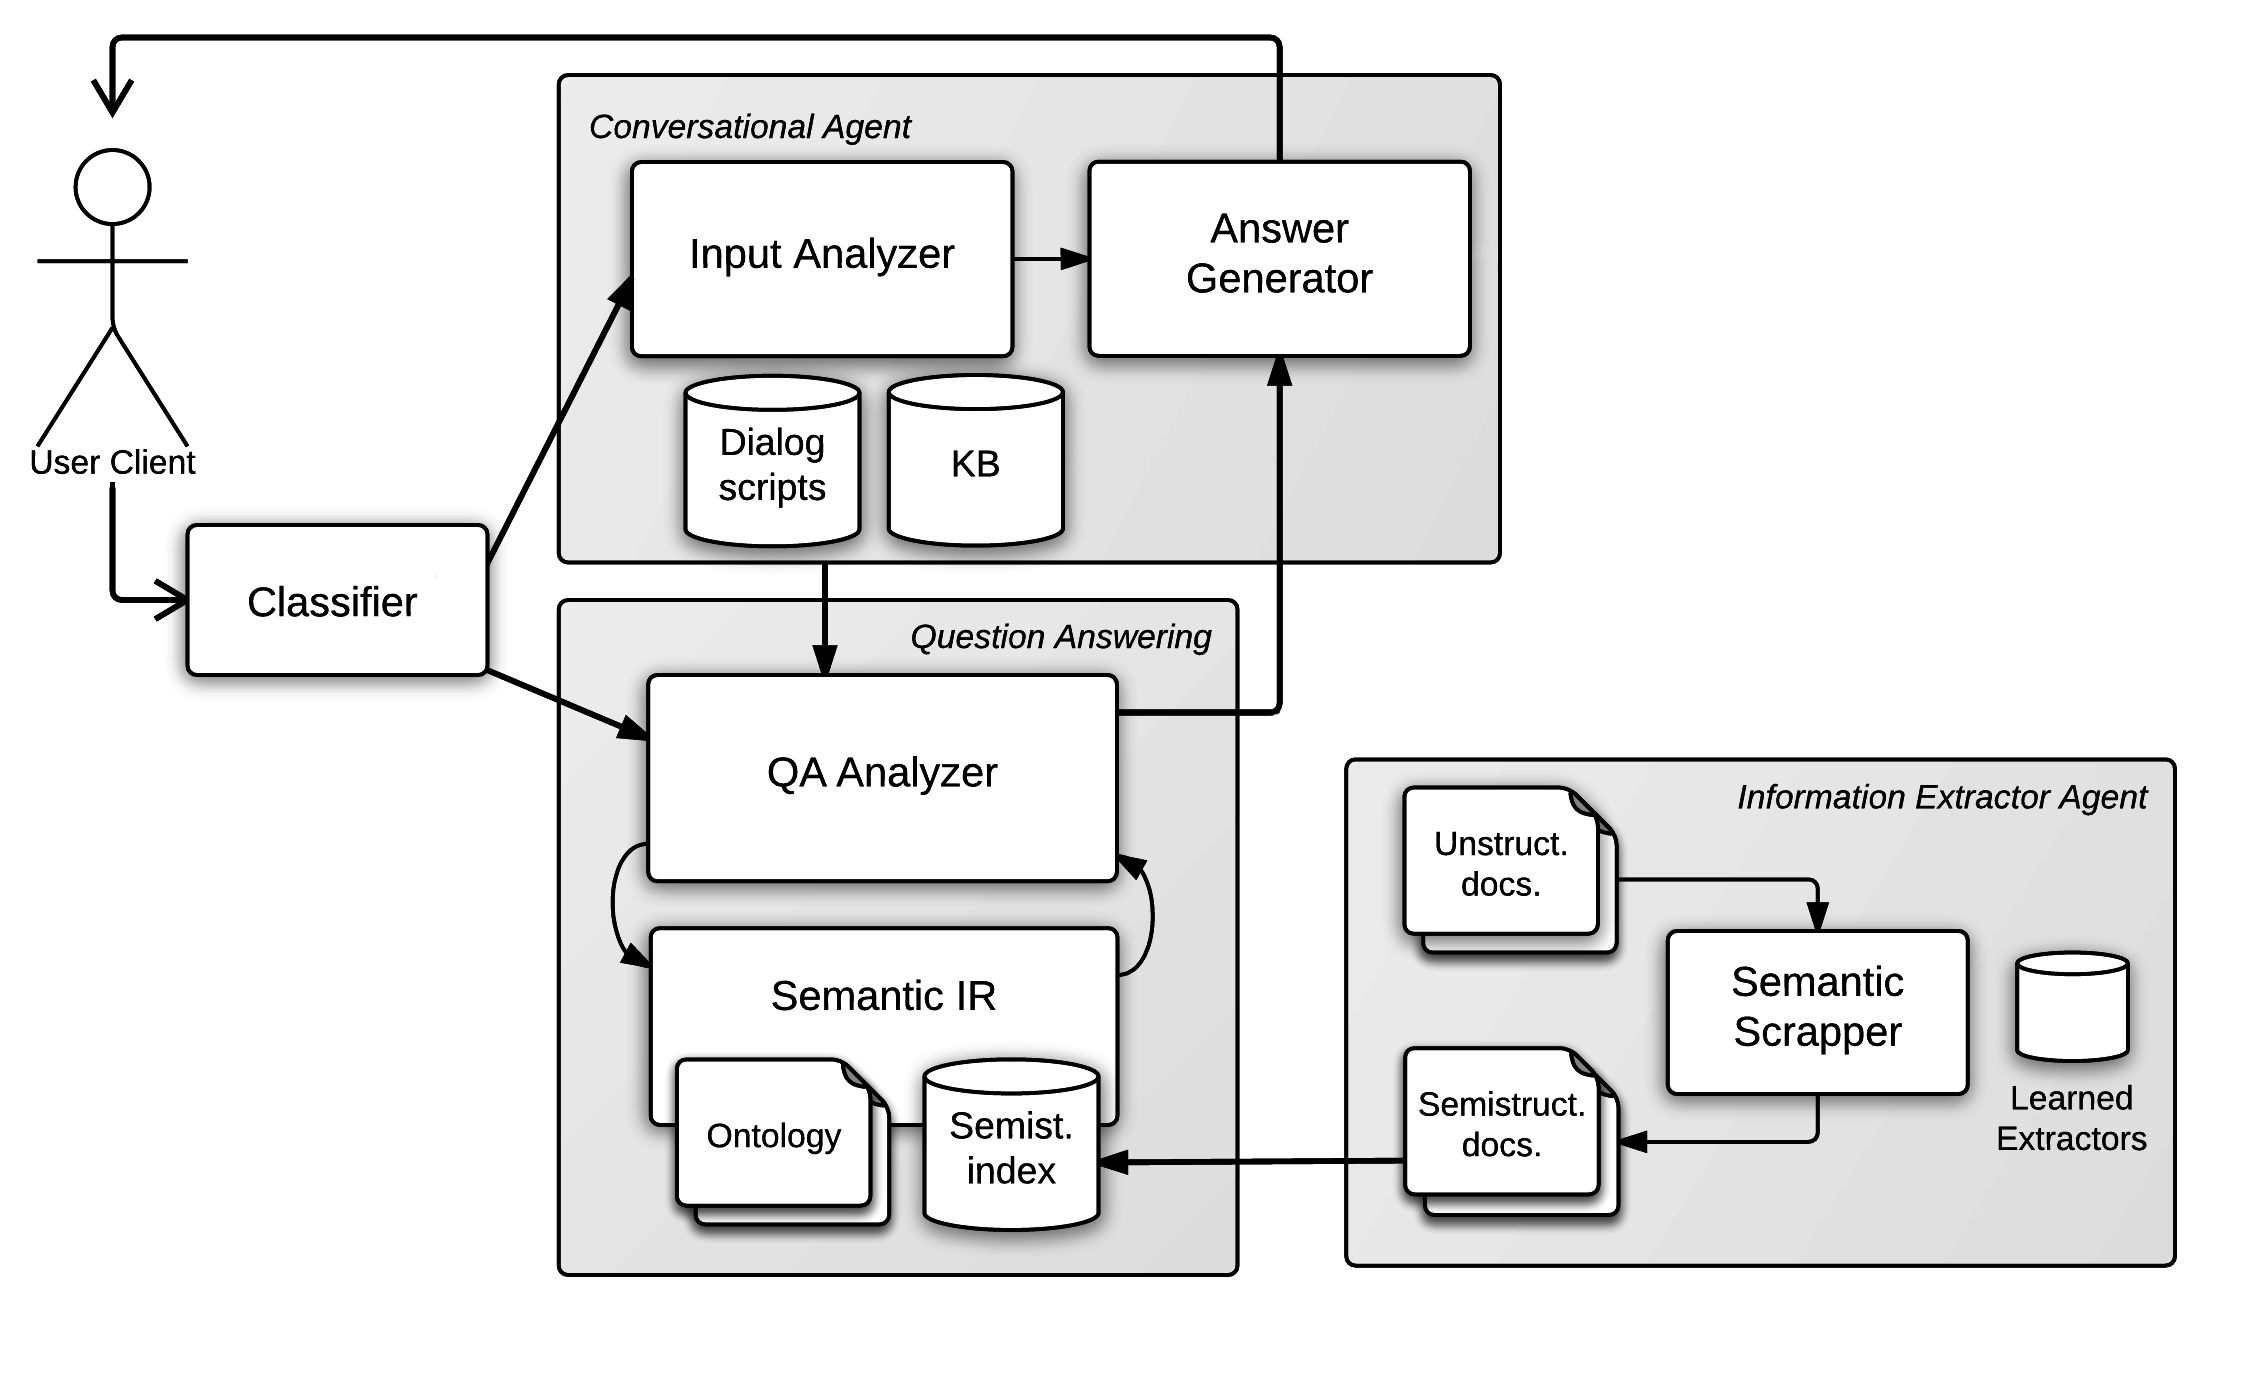
\includegraphics[width=0.7\textwidth]{img/arch/global_1-3.png}
    \caption{Global view of the architecture proposed}
    \label{fig:arch1}
\end{figure}



\subsection{Conversational Agent}

The {\em Conversational Agent} is responsible for handling the social dialog of the conversation (also referred by other authors as small talk or chit chat). It also traces the topic of the conversation that stores in the fact \ac{KB}, along with the former utterances and pills of information learned or devised from the user. It is responsible for understanding the whole meaning of the user query when he/she omits information already provided in previous utterances. 
The Input Analyzer inside the Conversational Agent, performs a script based analysis of the input by matching regular expressions against the input. Some advanced implementations of script based analyzers also use dictionaries and perform \ac{PoS} tagging and parsing.

The Conversational Agent, by means of the Answer Generator, is also in change of generating the answers that will be sent to the users. These are also stored in the dialog scripts. 
In the most common scenario, the small talk input is analyzed by the Input Analyzer and tells the Answer Generator to given a particular answer in response.
However, the \ac{QA} and the Teaching Agent modules can also instruct the Answer Generator to send a response to the user.
In those cases, the Conversational Agent generates the answer according to the topic and former utterances, giving it a particular touch when needed.
Besides the textual response that is presented to the user, the answer is decorated with metadata to provide further information about the state of the Conversational Agent. Typically, they indicate the mood of the agent, its facial expressions and gestures (possible implemented using \ac{BML}), etc.


\subsection{Question Answering}

The {\em Question Answering} takes part with those user queries where he/she asks for a particular piece of information, i.e. as with a regular \ac{QA} system. 
The QA Analyzer uses domain-specific grammars to extract the precise meaning of the query.
This is, it is classifies the type of query, extracts the relevant concepts, and categorize them according to the ontologies considered. The effectiveness of the process depends of the accuracy and degree of detail of the grammars applied, which includes the precision of the concept categorization. The QA Analyzer combines general-scope dictionaries with domain-specific ones to enhance its effectiveness. If there is no grammar that can be applied to the query, the analysis simply does not return any outcome.

As with regular \ac{QA} systems, the \ac{IR} is consulted to obtain the relevant documents where the answer is contained. The \ac{IR} works with a set of documents that has been previously indexed.
% Once the user query is analyzed the system decides whether the system needs to query the available document in order to retrieve the information to generate the results. 
In this case, given the semantic nature of the \ac{IR} system, it also acts as a SPARQL endpoint that may be queried for precise pieces of information. Thus, it supports a dual working mode depending on the nature of the query. 
With semantic queries the results are more precise and the information returned has better structure, the better categorization of the fields returns the more accurate results. 
Semantic queries also enable the use of linked data not only for enhancing results but for query expansion.
% {\bf search som QueryExpansion papers or review those at mendeley}. 
When the semantic IR is not available --either because the incoming query is too general, or because there is no relevant structured documents--, the IR module will do its best to return a piece of information as accurate as possible. At least, it retrieves a set of documents that are related to the query. It will try to categorize the nature of the documents, which bring the category of the concept searched, that can be used to expand the query and reformulate the query.
%  The main advantage of including semantic IR is that it will provide a result, depending on the quality of the documents, the quality of the result may vary, but in most cases (but when there is no relevant document at all) it will produce a result.
If no relevant document is returned by the \ac{IR}, the \ac{QA} is not capable to give a response, and thus the Answer Generator will inform the user. 

Moreover, the Semantic \ac{IR} may also be queried by external modules, e.g. the Teaching Agent. The treatment given to the query is the same as when it comes from the QA Analyzer.
Finally, the conversational agent may derive a query to the \ac{QA} in those cases where the Speech Act Classifier missclassifies the query, and more frequently with those utterances where the user	 asks for more information. In this case, the \ac{QA} system needs further information to perform the document retrieval. Thus, the conversational agent will expand the query and route it to the \ac{QA}.


\subsection{Information Extractor}

In case there is no relevant document for the query performed, the system will try update the KB. The {\em Information Extractor Agent}'s main function consists on analyzing unstructured documents in order to extract fields, categorize them and generating a semistructured document. 

This is a slow process, so it cannot be performed in near real-time; instead, unresolved query may trigger its execution, that will be available for future queries. 
This automatic information extraction mechanism is a best-effort process that relies on the information on the sources, and the ontologies used to map that information. Semantic scrappers such as Scrappy~\cite{villamor13} may boost this process.
Alternatively, a system administrator may also manually include documents on the \ac{IR} index, but also mark them to be processed by the Information Extractor Agent and index them afterwards.

\subsection{Teaching agent}

The {\em Teaching Agent} supervises the learning process of the users, and is in charge of improving their learning experience.
To do so, it  gathers information about all interactions of the user with the system. This information is obtained from the \ac{KB} of the Conversational Agent (or derived from it) which is synchronised with the Student Profile KB of the \ac{ITS}.
An \ac{ITS} is usually implemented as a \ac{MAS} of \ac{BDI} agents. In that case, the Student Profile KB is included in the \ac{BB} of the agent. 

% I don't really know if this should go here or not...
%\section{Prototype}
%
\section{Work process} % Revise this title

In this section we will describe the process a question introduced into the system will follow. Depending on the user input, the aforementioned process may differ. Here, we will consider two types of user input, the first one being a simple chit chat sentence, that won't require a look up in the \ac{KB}. The other type of input to be considered is an actual question, requiring a lookup in the \ac{KB}.

% Add UML figure?

The classifier will differentiate between the different types of input, and trigger the appropriate processes.

\subsection{Simple sentence}

Our system is ready to handle social chat, which aims to provide a richer experience to the user, encouraging him to keep chatting and having a better learning experience. In this case, a \ac{KB} lookup is not required, and therefore, the process is as stated:

\begin{enumerate}
 \item The user inputs the sentence into the system.
 \item The classifier tags the input as chit-chat.
 \item The input analyzer decides which type of social interaction we are facing, such as a greeting, a identifying question (``Are you the teacher? `` ) or an insult, among others.
 \item The answer generator provides an appropriate response and returns it to the user.
\end{enumerate}

This process is shown graphically in Figure \ref{fig:arch2}

\begin{figure}[!htbp]
    \centering
    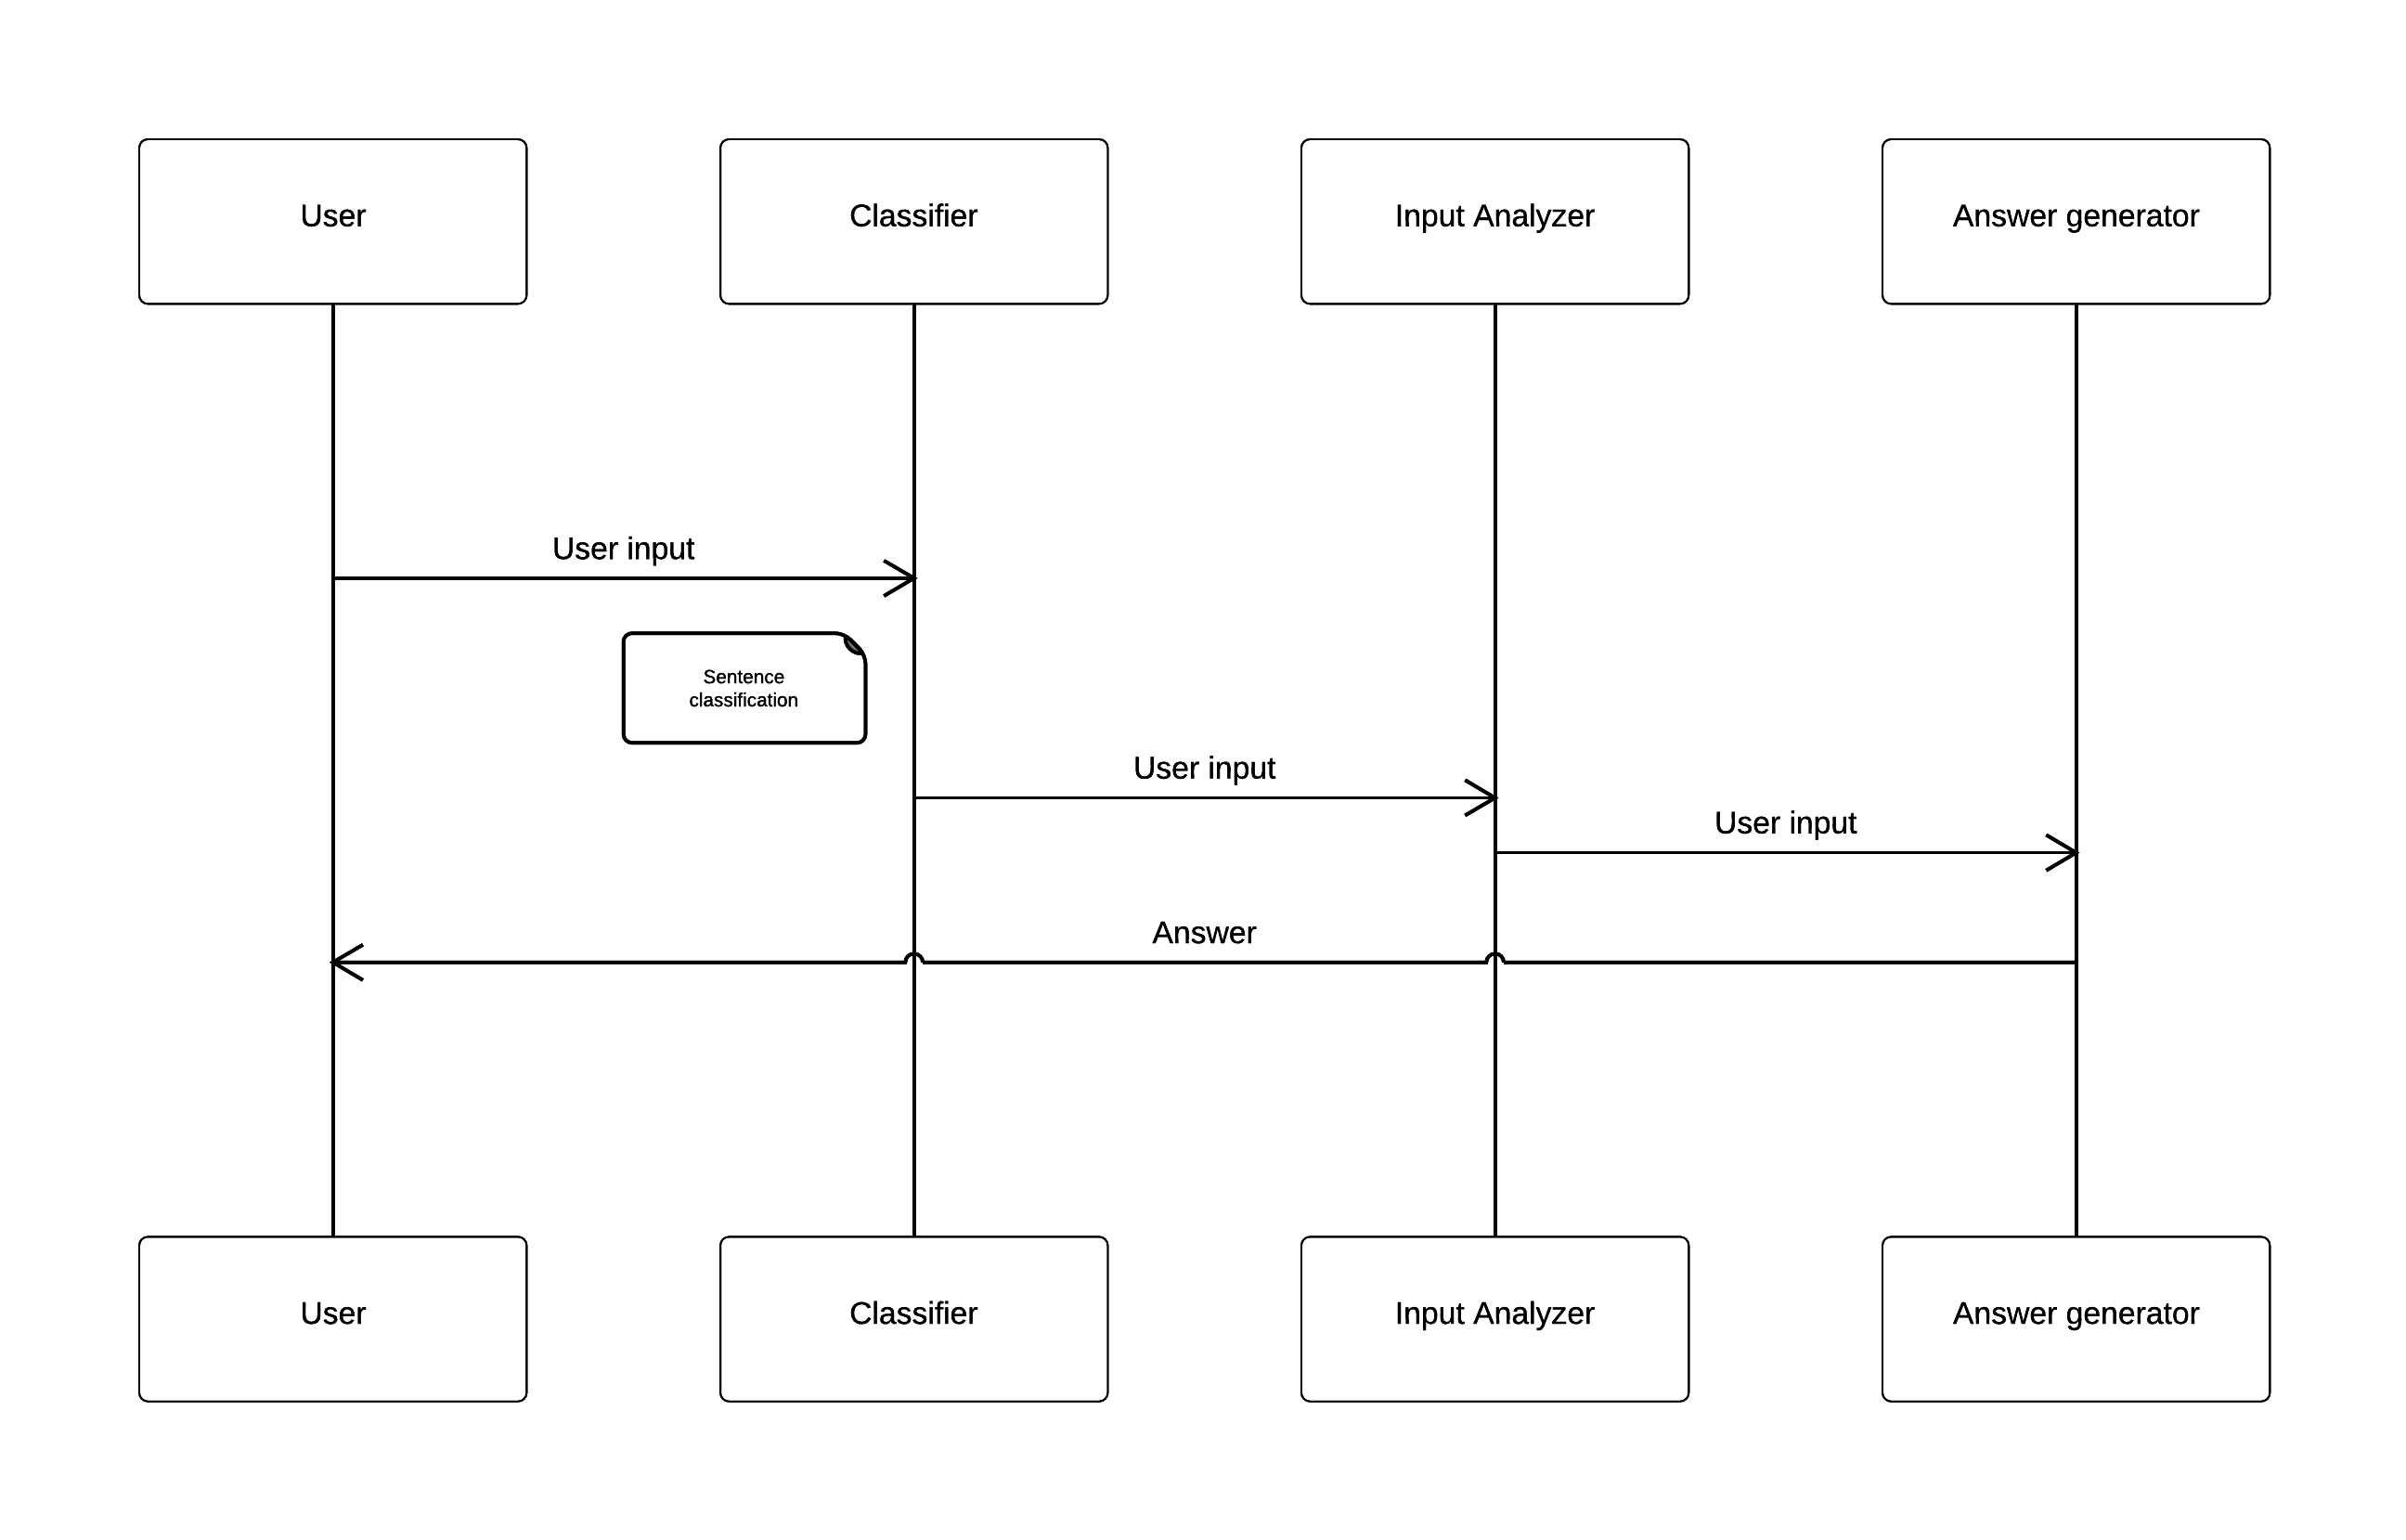
\includegraphics[width=\textwidth]{img/arch/SimpleSentence.png}
    \caption{Simple sentence process}
    \label{fig:arch2}
\end{figure}

\subsection{Question with \ac{KB} lookup}

In this process, the question input into the system does require a lookup in the \ac{KB}, via the \ac{QA} system. The process followed to produce the output will be the following:

\begin{enumerate}
 \item The user inputs the question into the system.
 \item The classifier tags the input as an actual question.
 \item The QA Analyzer process the question and performs a search in the \ac{KB}.
 \item The QA Analyzer returns the response for the question to the Answer generator.
 \item The answer generator process the response and returns a natural question, as well as the required \ac{OoB} command with the data.
\end{enumerate}

Figure \ref{fig:arch3} shows the process graphically.

\begin{figure}[!htbp]
    \centering
    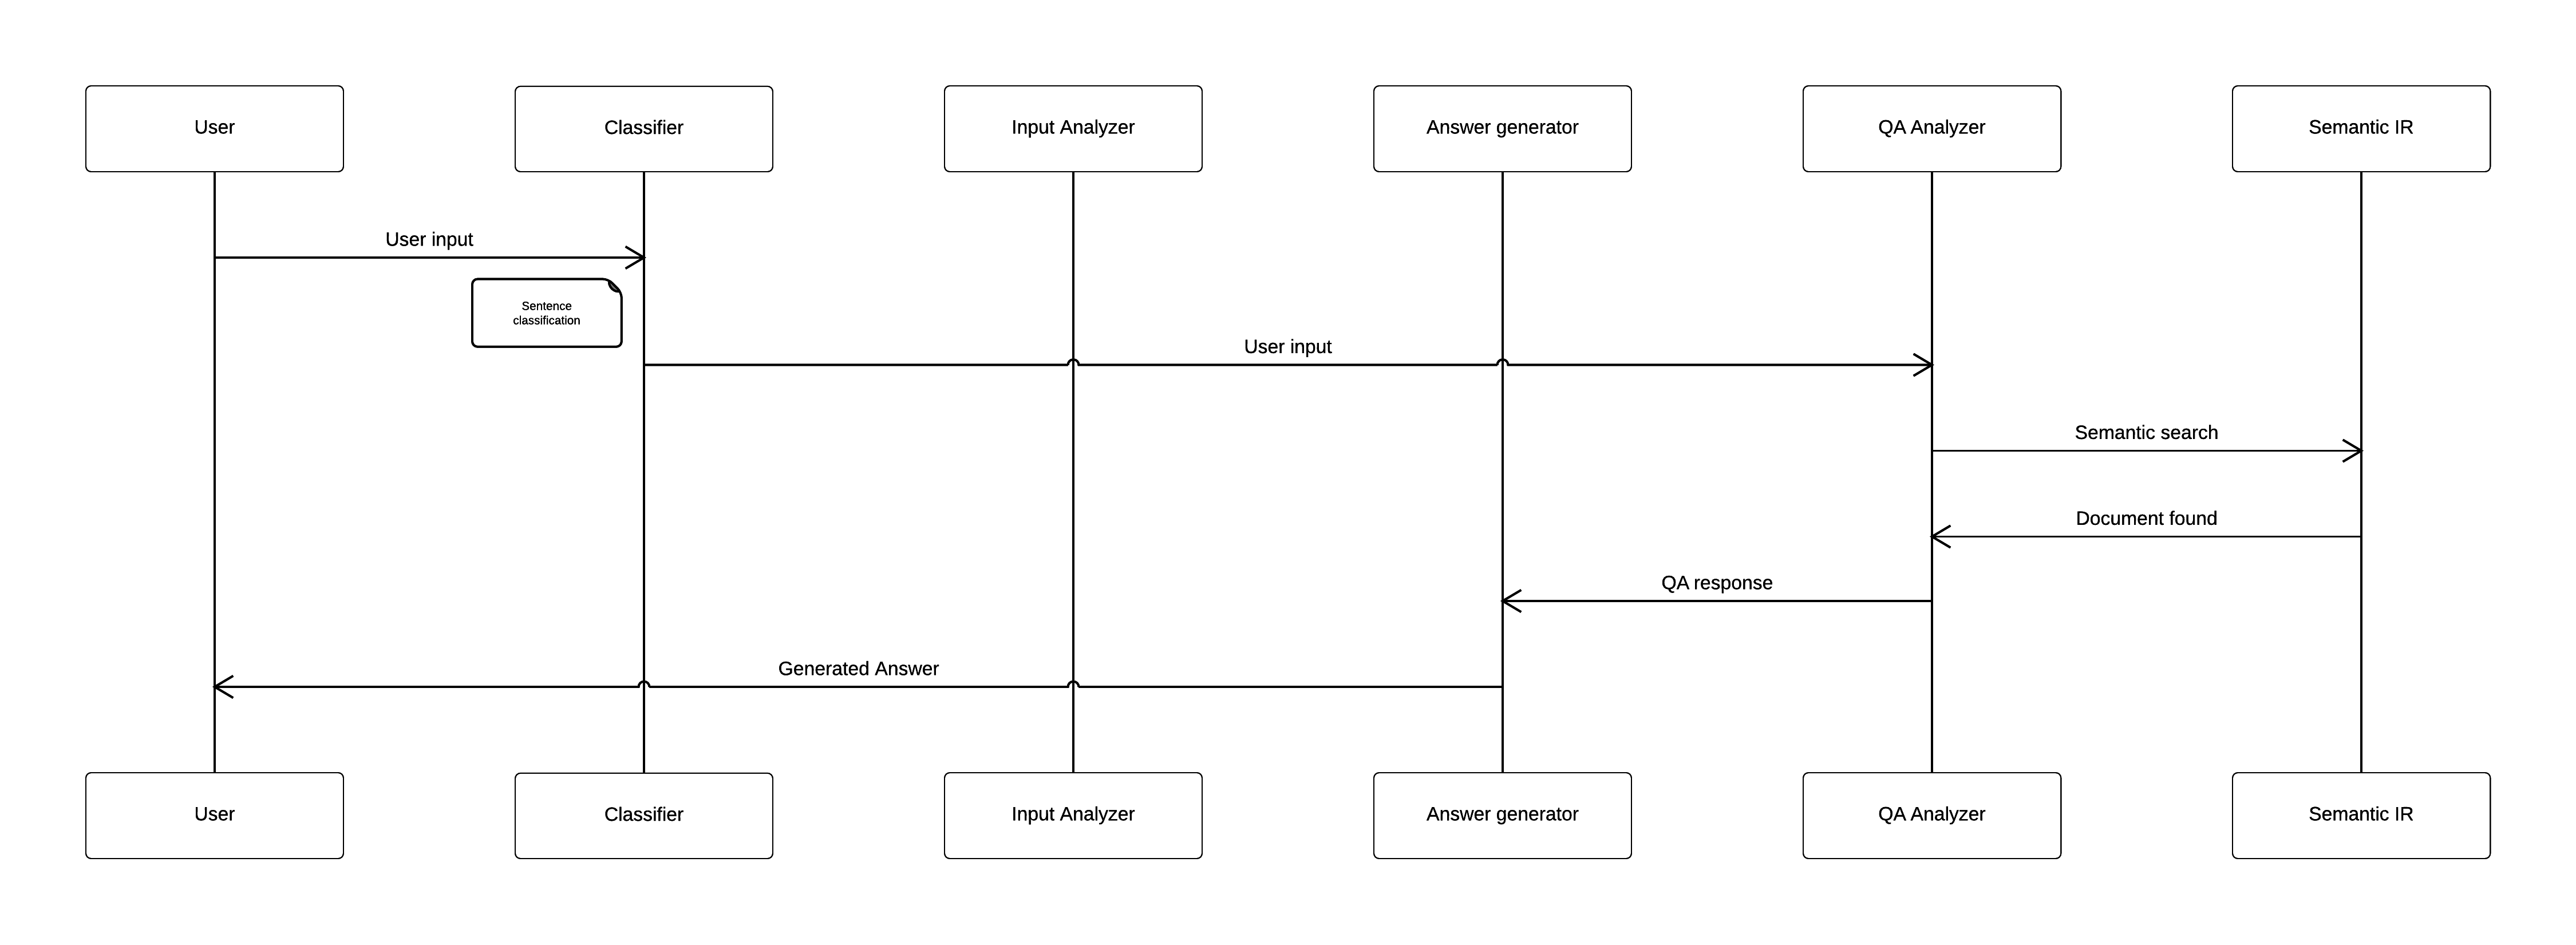
\includegraphics[width=\textwidth]{img/arch/FullQuestion.png}
    \caption{Question with \ac{KB} lookup process}
    \label{fig:arch3}
\end{figure}

% 
% Several things should go here:
%  * A description of how the system will behave when a question is received
%  * An UML (or several) describing that behaviour
%  * Something about PoS ?
\chapter{Prototype}
\label{chap:prototype}

\begin{chapterintro}

In this chapter, we will describe the prototype we developed following the architecture described in the previous chapter. We will start with a short overview of the implemented modules for the system, to then take a detailed look to each one of them, describing how they work, and how they connect to each other.
 
\end{chapterintro}

\cleardoublepage

\section{Overview of the system}

For this system, we developed a prototype utilising the architecture explained in chapter \ref{chap:architecture}. To do so, we deployed the following modules and subsystems:

\begin{enumerate}
 \item A Javascript client, that will connect to the system and act as an user interface.
 \item A Front-end controller, written in python, that will handle the interaction between the different modules-
 \item A chatbot using chatscript, to handle question analysis and chit-chat interaction.
 \item An Apache Solr instance, where all the semantic data will be loaded.
\end{enumerate}

In parallel to all this, both a web scraper using scrapy to recover the relevant data, and an uploader to post the data to Solr.

\subsection{Chat client}
\label{sec:chatclient}

In our prototype, the interaction with the system is done via a web client that provides a chat box and an iframe where the content is located. When the user first opens the page, it's greeted by the bot, and provided with a   short explanation of how the client works.

\begin{figure}[!htbp]
    \centering
    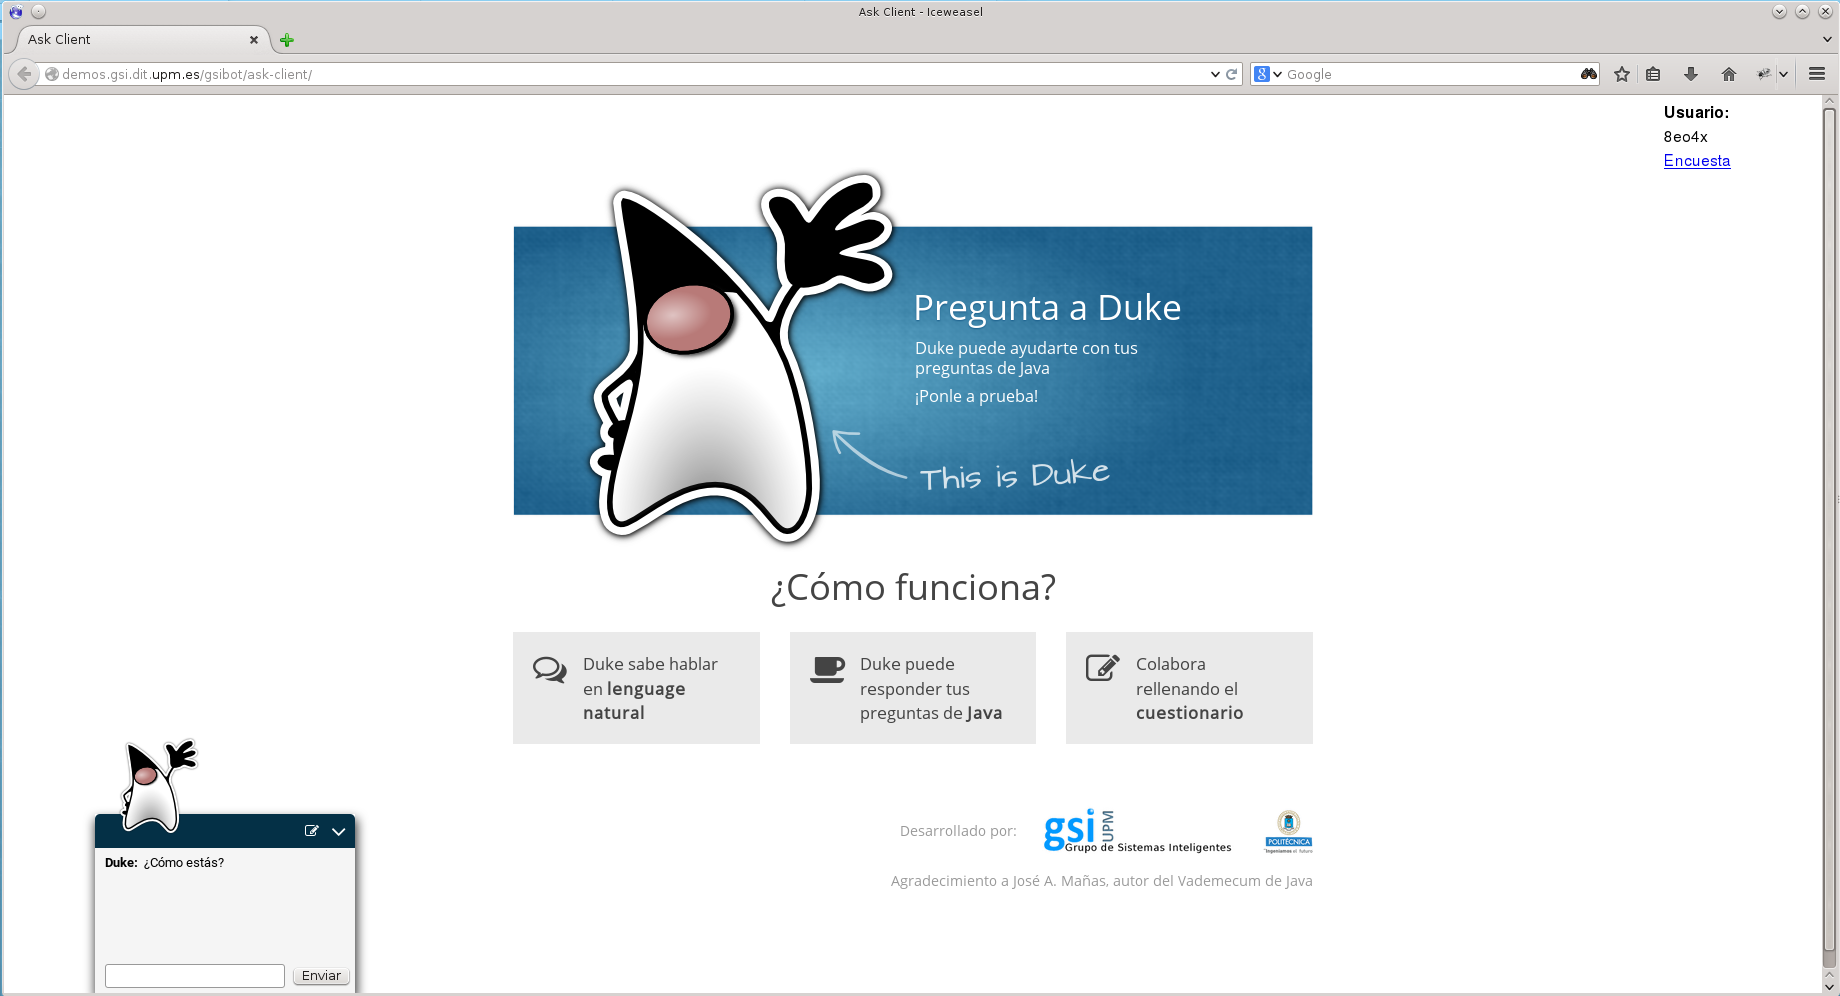
\includegraphics[width=0.7\textwidth]{img/screens/ask-client.png}
    \caption{Web interface for the client.}
    \label{fig:chat1}
\end{figure}

The client is made using web technologies: HTML, CSS and Javascript, and uses Ajax to communicate with the server sending the user questions and handling the response, waiting for the user to send a question and then making the request to the server, as shown in listing \ref{listing:formclient}.

%\emph{\textcolor{red}{Add example of JSON request? Add html code?}}

\begin{center}
  \lstinputlisting[language=JavaScript, caption=Ajax performing the request to the controller, label=listing:formclient, firstline=77, lastline=118]{code/prot/ask.js}
\end{center}

Upon the user submitting a question through the interface, the client will send a GET request to the controller, as described in section~\ref{sec:frontendcon}, and will receive a json response, containing the answer and the page to be shown to the user, if existent. An example response to que question ``¿Qué es un for?'' is shown in listing~\ref{listing:jsonchatresponse}.

\begin{center} 
  \begin{lstlisting}[language=json, caption=Example response for the chat client, label=listing:jsonchatresponse]
   {
     "answer": [
		"Esto es lo que s\u00e9 sobre for",
		"Si quieres, creo que bucles for degenerados tienen algo que ver con esto"
	       ],
     "definition": "Los bucles for se ejecutan un n\u00famero determinado de veces",
     "links": [
                "http://www.dit.upm.es/~pepe/libros/vademecum/topics/3.html",
                "http://www.dit.upm.es/~pepe/libros/vademecum/topics/139.html",
                "http://www.dit.upm.es/~pepe/libros/vademecum/topics/140.html",
                "http://www.dit.upm.es/~pepe/libros/vademecum/topics/141.html",
                "http://www.dit.upm.es/~pepe/libros/vademecum/topics/142.html",
                "http://www.dit.upm.es/~pepe/libros/vademecum/topics/143.html"
                ] ,
     "resource": "http://www.dit.upm.es/~pepe/libros/vademecum/topics/138.html"
   }  
  \end{lstlisting}
\end{center}

\subsection{Front end controller}
\label{sec:frontendcon}
The Front end controller is the main control module in our system. It handles the requests received from the client described in \ref{sec:chatclient}, and proceeds to triggers the required modules, as well as executing the \ac{OoB} commands received from each module. This module is provided as a web service, and therefore we have chosen Flask~\cite{flask0101} and Apache's mod\_wsgi~\cite{modwsgi} to deploy it. In the following subsections we will describe how it works as well as its work-flow structure.

\subsubsection{Functional Model}

The function of this module is returning the answer to the user, formed as JSON, by triggering the appropriate modules and reacting to their responses. To do so, it follows a process explained in the UML diagram shown in Figure \ref{fig:fe-model1}.

\begin{figure}[!htbp]
    \centering
    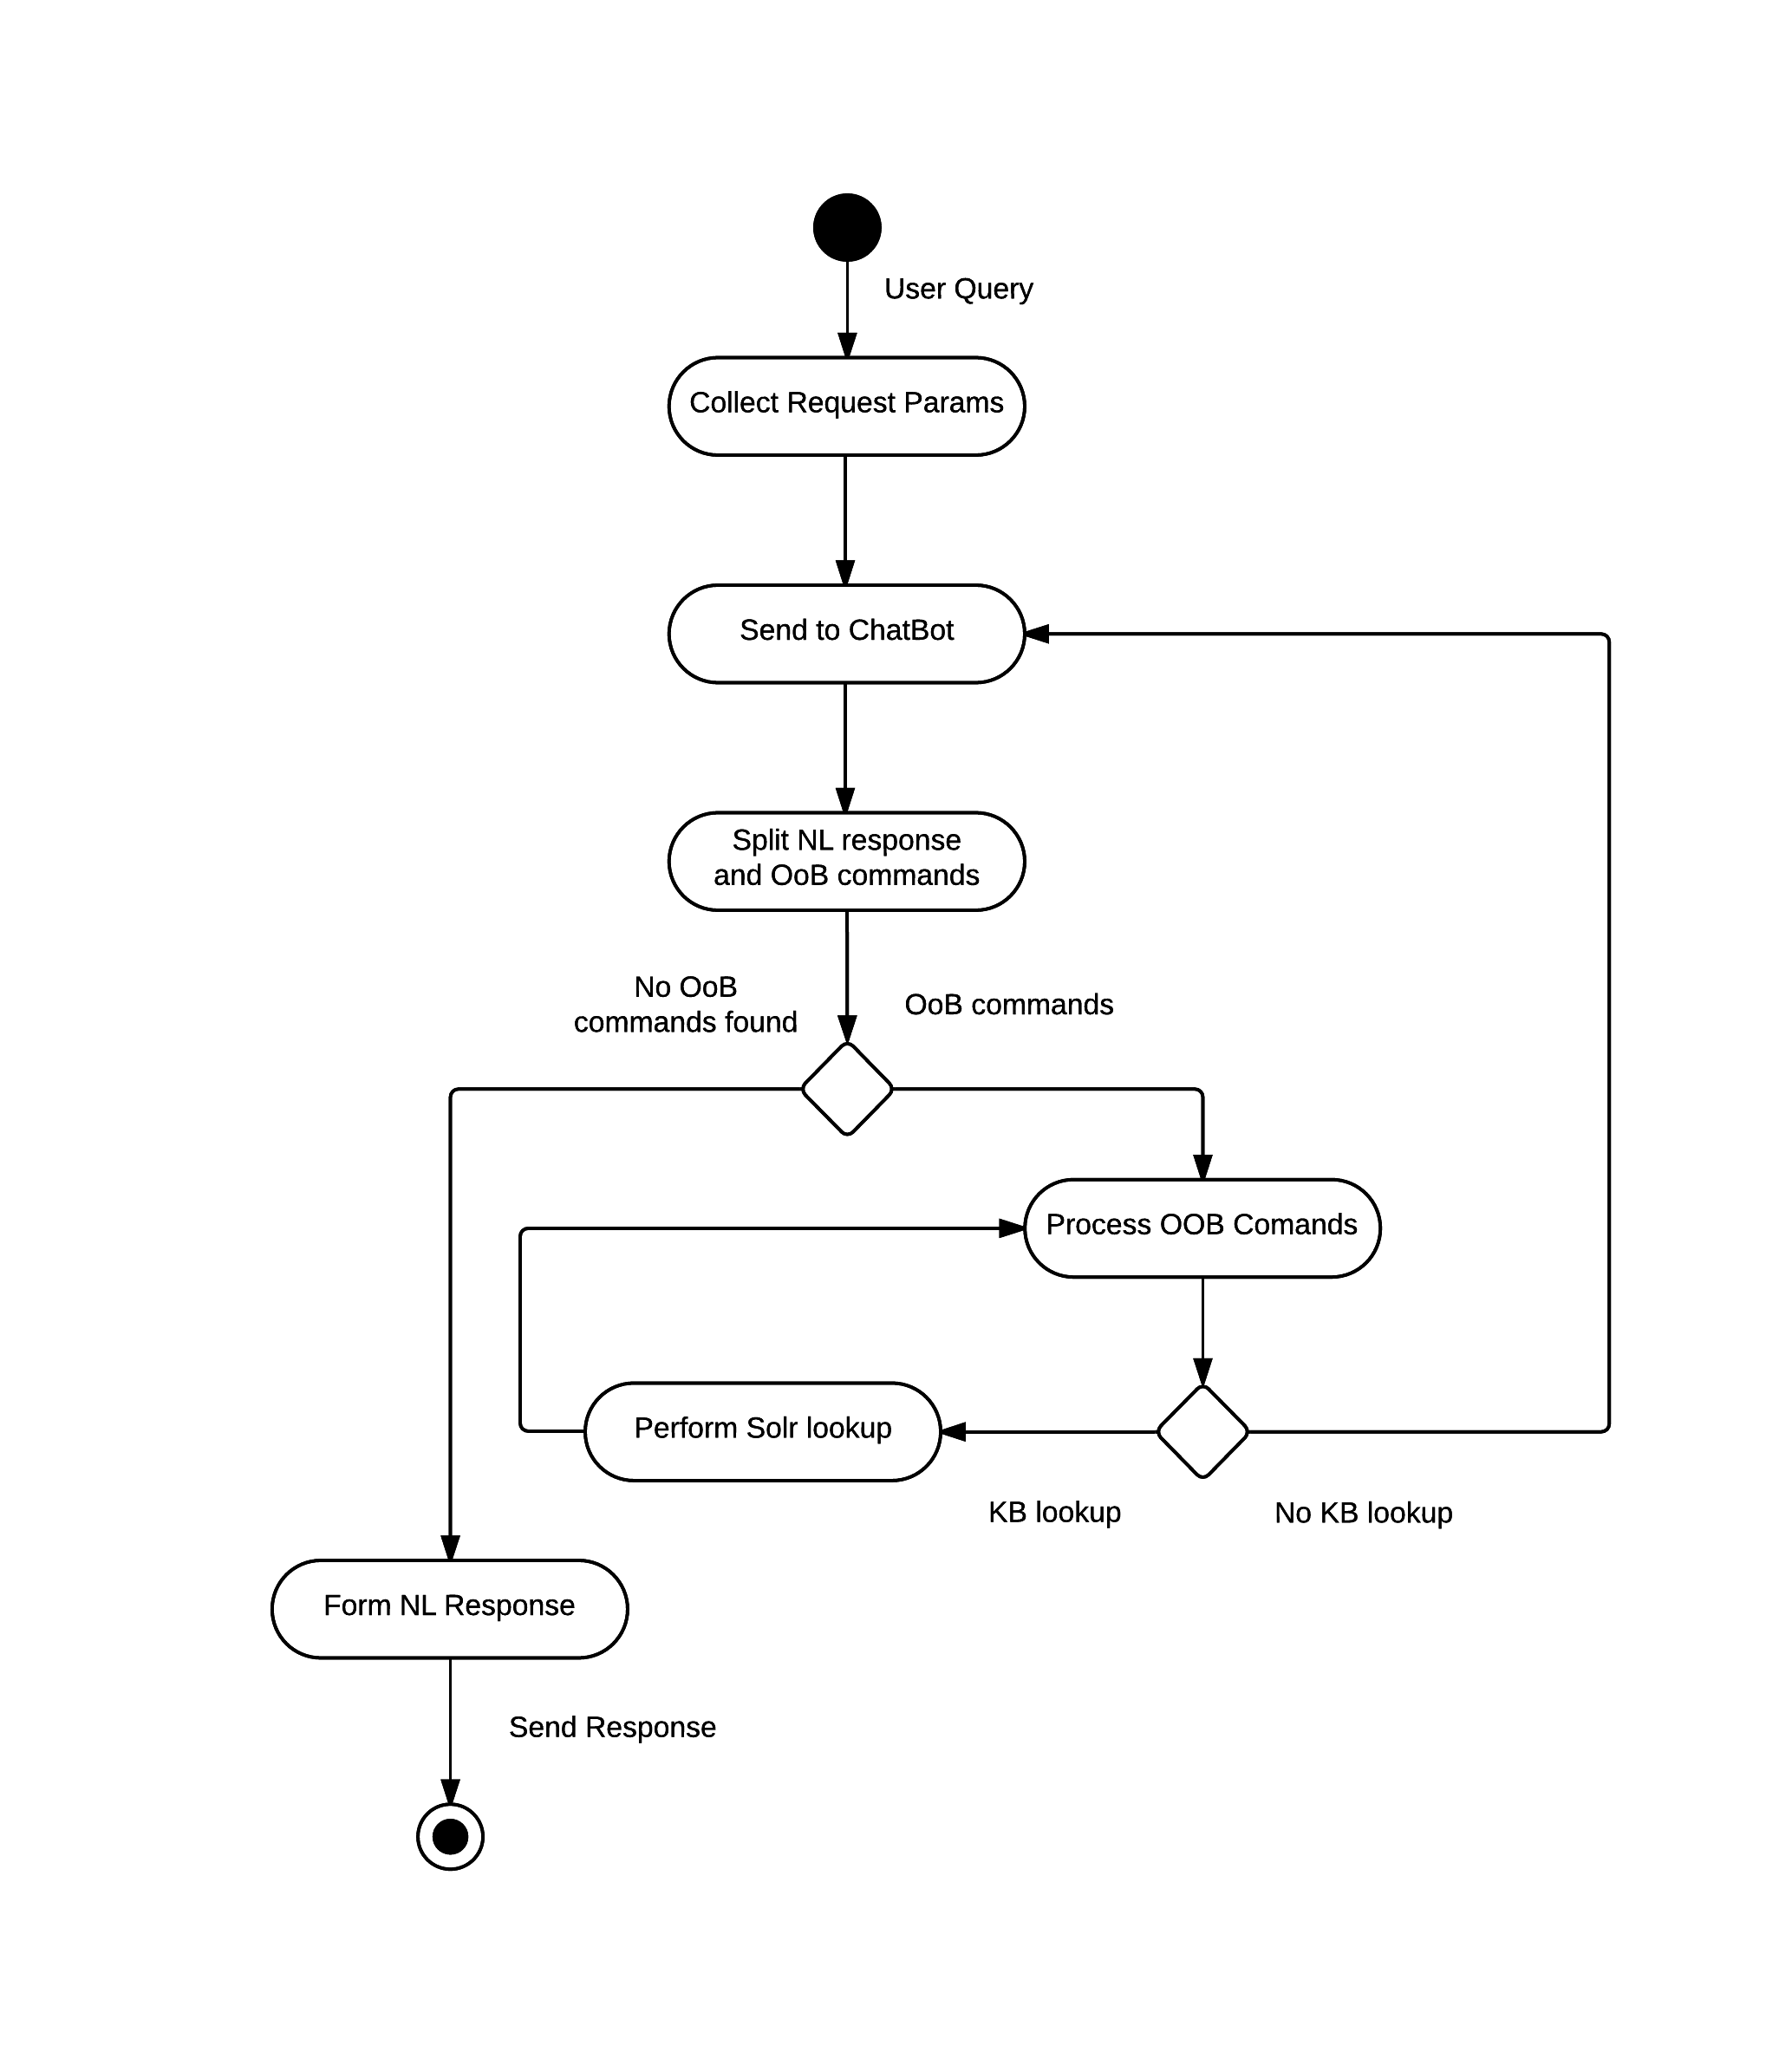
\includegraphics[width=0.8\textwidth]{img/prot/activityDiagram.png} 
    \caption{UML diagram of the process followed by the controller.}
    \label{fig:fe-model1}
\end{figure}

\begin{itemize}
 \item \textbf{Request parsing:} The client sends the query as JSON using a HTTP request to the front-end controller. This JSON is recovered and processed into a python dictionary.
 \item \textbf{Send to ChatBot:} The user query is sent to the ChatBot so it's processes and a response, either \ac{NL} or \ac{OoB}, is generated.
 \item \textbf{Split \ac{NL} response and \ac{OoB} commands} The response in the previous step is split in \ac{NL} and {OoB} commands, to process each one appropriately.
 \item \textbf{\ac{OoB} command processing:} Read the \ac{OoB} commands and take the appropriate steps for each one of them.
 \item \textbf{Solr Lookup:} If a lookup in the Knowledge base is required, send the query to Solr.
 \item \textbf{Form Response:} Once there are no more \ac{OoB} commands, form the actual response in JSON and send it to the user.
\end{itemize}

% Add the workflow of the controller.

\subsubsection{Structural Model}

In this section we will describe the structure followed designing the front end controller. In figure \ref{fig:fe-methods1} we show the method structure of the controller.
\begin{figure}[!htbp]
    \centering
    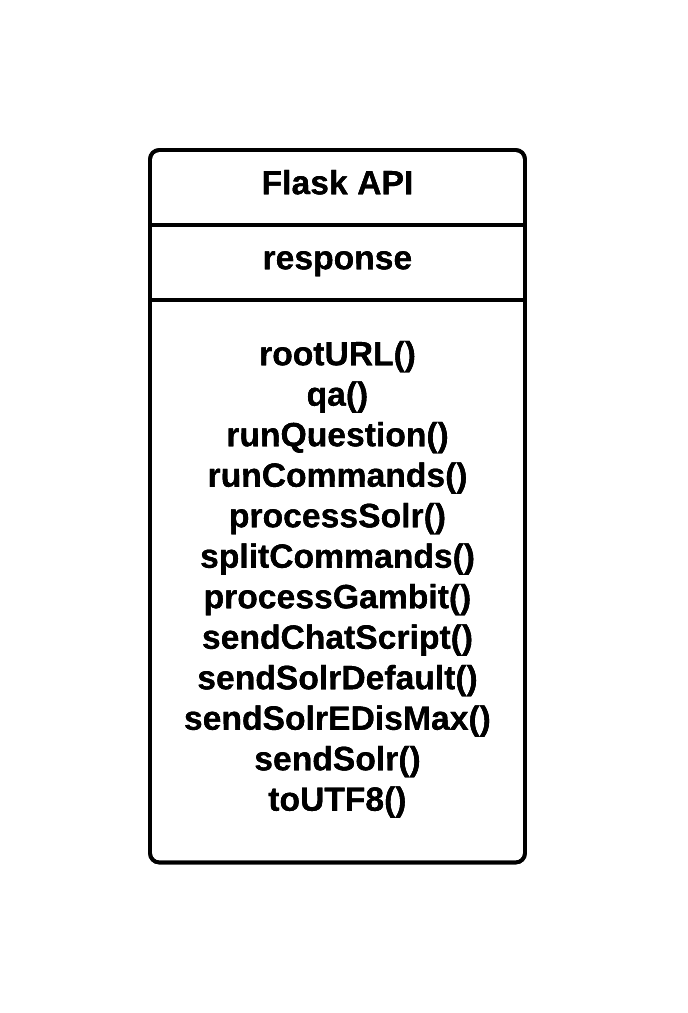
\includegraphics[width=0.4\textwidth]{img/prot/controllerStructure.png}
    \caption{Front end controller structure}
    \label{fig:fe-methods1}
\end{figure}

Now we will proceed to describe each of the methods shown in the figure.

\begin{itemize}
  \item \textbf{rootURL()} will be triggered whenever the base URL for the controller is requested. It will act in the same way than the qa() method.
  \item \textbf{qa()} this function will recover the request parameters, shown in table \ref{tab:fe-qparams}, and start the process to understand the user query, in order to return the appropriate response, whose parameters are shown on table \ref{tab:fe-rparams}.
  \item \textbf{runQuestion()} in this function, we will simply run the question once throught ChatScript, and then start the main command processing.
  \item \textbf{runCommands()} Given the \ac{NL} response from ChatScript, it will split the \ac{OoB} commands and start processing each one of them, as well as their responses, adding commands to the queue as needed.
  \item \textbf{processSolr()} For the solr command, this method will construct the solr query, and keep sending it to Solr increasing its fuzziness level, until an answer is found, or a maximum fuzziness is reached, in which case it will return the empty solr response.
  \item \textbf{splitCommands()} Taking a \ac{NL} sentence as a parameter, this method will return both a list with all the \ac{OoB} commands in the sentence, as well as the \ac{NL} part of the sentence, or an empty string if the sentence was made only of \ac{OoB} commands. 
  \item \textbf{processGambit()} when a direct search does not return any answer, the system will perform a broader search in Solr. This is further explained in section \ref{sec:solr}.
  \item \textbf{sendChatScript()} This function will process the interaction with ChatScript, both sending the questions and handling the responses. For more details, see section \ref{sec:chatbot}.
  \item \textbf{sendSolrDefault()} Given a question and no other parameters or information, this function will send said question to Solr, so it will go through the default processing. This is mainly unused.
  \item \textbf{sendSolrEDisMax()} When a gambit is needed, send the question to Solr using an \ac{eDisMax} query, which will search in different fields, valuing each field using a given weight. 
  \item \textbf{sendSolr()} Used by the rest of the Solr related methods, this function will handle sending the payload given as parameter to Solr, and returning the JSON response.
\end{itemize}

\begin{center}
  \begin{table}
    \begin{tabular*}{0.7\textwidth}{@{\extracolsep{\fill}} | c | c | p{0.5\textwidth} |}
      \hhline{|-|-|-|}
      \textbf{Parameter} & \textbf{Name} & \textbf{Description} \\ \hhline{|=|=|=|}
      question & User's question & The question submitted by the user. \\ \hhline{|-|-|-|}
      bot & Bot & The bot the query will be send to. \\ \hhline{|-|-|-|}
      username & The user & A random identifier for the user communicating with the bot. \\ \hhline{|-|-|-|}
      \end{tabular*}
    \caption{Parameters in the query received by the front end controller.}
    \label{tab:fe-qparams}
  \end{table}
\end{center}

\begin{center}
  \begin{table}
    \begin{tabular*}{0.7\textwidth}{@{\extracolsep{\fill}} | c | c | p{0.5\textwidth} |}
      \hhline{|-|-|-|}
      \textbf{Parameter} & \textbf{Name} & \textbf{Description} \\ \hhline{|=|=|=|}
      Answer & The Bot's response & The \ac{NL} response generated by the bot. \\ \hhline{|-|-|-|}
      Resource & An URL & The url of the relevant document where the information is, if existent. \\ \hhline{|-|-|-|}
      \end{tabular*}
    \caption{Parameters in the query sent back to the client.}
    \label{tab:fe-rparams}
  \end{table}
\end{center}

Finally, we will describe the \ac{OoB} commands that the system will be able to process.

\begin{itemize}
 \item \textbf{¬sendSolr} this command is issued whenever a question matches the pattern specified to request information about a Java topic.
 \item \textbf{¬solrResponse} after a search is performed in Solr, this command is issued to indicate whether or not a response has been found, and returning said response.
 \item \textbf{¬solrLinks} a special Solr search, looking for related topics in Solr.
 \item \textbf{¬solrLinksResponse} as a response to the solrLinks command, returns a list with the related topics.
 \item \textbf{¬gambit} perform an \ac{eDisMax} search in Solr, using the full user question.
 \item \textbf{¬gambitResponse} returns the title of the most relevant document found in the \ac{eDisMax} search.
 \item \textbf{¬gambitUnknown} issued when no document with a high enough score is found in Solr.
 \item \textbf{¬resource} sets the url to be displayed in the final response returned to the client.
 \item \textbf{¬label} sets the title of the found document as the label for the response.
\end{itemize}

The syntaxes of the commands is specified in table \ref{tab:oob-commands}.
\begin{center}
  \centering
  \begin{table}
    \begin{tabular*}{0.7\textwidth}{@{\extracolsep{\fill}} | c | c | p{0.35\textwidth} |}
      \hhline{|-|-|-|}
      \textbf{Command} & \textbf{Syntaxes} & \textbf{Description} \\ \hhline{|=|=|=|}
      ¬sendSolr & ¬sendSolr \textit{reqfield} \textit{doctitle} & Searchs in solr for the \textit{doctitle} and returns the \textit{reqfield} field.  \\ \hhline{|-|-|-|}
      \multirow{2}{*}{¬solrResponse} & ¬solrResponse \textit{unknown} & The requested document was not found in Solr. \\ \cline{2-3}
				     & ¬solrResponse \textit{reqfield} \textit{response} & Returns as \textit{response} the data of the field \textit{reqfield}. \\ \hhline{|-|-|-|}
      ¬solrLinks & ¬solrLinks \textit{linklist} & Asks for a search in Solr for the name of the topics given as an uri in the linklist \\ \hhline{|-|-|-|}
      ¬solrLinksResponse & ¬solrLinksResponse \textit{nameslist} & Sets the response for the ¬solrLinks command, returning the first name of the links. \\ \hhline{|-|-|-|}
      ¬gambit & ¬gambit \textit{topic}& Asks for a \ac{eDisMax} search on Solr, passing the full question. \\ \hhline{|-|-|-|}
      ¬gambitResponse & ¬gambitResponse \textit{gambittopic} & After performing an \ac{eDisMax} search, returns \textit{gambittopic} as the suggested topic. \\ \hhline{|-|-|-|}
      ¬gambitUnknown & ¬gambitUnknown & After performing an \ac{eDisMax} search, indicates that no relevant document has been found. \\ \hhline{|-|-|-|}
      ¬resource & ¬resource \textit{URL} & Sets \textit{URL} as the resource to be displayed in the client \\ \hhline{|-|-|-|}
      ¬label & ¬label \textit{topic} & Sets \textit{topic} as the concept of the response \\ \hhline{|-|-|-|}
      \end{tabular*}
    \caption{Parameters in the query sent back to the client.}
    \label{tab:oob-commands}
  \end{table}
\end{center}

\subsection{ChatBot}
\label{sec:chatbot}

The ChatBot handles the processing of the natural language input from the user, and controls the conversation. To do so, it uses the chat engine ChatScript, described in section \ref{subsec:chatscript}. We will first describe the ChatBot rules, and how they process the user input, and then proceed to describe how to launch and communicate with the ChatScript server.

\subsubsection{The rules}

Chatscript responds to a series of rules, specified in its topic files. This rules will match the user input and produce an appropriate response, or output a rejoinder if no rule is matched. A more in depth description of how chatscript rules work can be found in section \ref{subsec:chatscript}.

We have separated our topics across several files, each containing related topics, as well as the control script for the bot. We will start describing the control process, shown in listing~\ref{listing:cs-control}

\begin{center}
  \lstinputlisting[language=C++, captionpos=b, caption=Control process for ChatScript, label=listing:cs-control, firstline=16, lastline=80]{code/prot/control.top}
\end{center}

In this process, we first check if we are currently in any conversation and have any pending rejoinders ready to match the output. Then proceed to check for rules looking for matches in the JAVA and EJEMPLOS topics. If no answer is provided, we will look for gambits and proper responses in the current topic, and then in the rest of the topics with keywords associated. In the case no match have been found yet, the user input will be test against the keywordless topic, looking for both responses and gambits, and, finally, if there is still no response, a generic answer will be provided, asking the user to modify its question.

As we have just mentioned, there are several topics, both with and without keyword, spread across several files, containing both said topics and the sets of concepts used in the bot. This files and the topics contained in them are:

\begin{itemize}
 \item \textbf{topic.top} This file has most of the concepts used in the other files, as well as three generic topics:
 \begin{itemize}
  \item \emph{TENCUESTA} to answer questions regarding the poll that will be presented to the user.
  \item \emph{EXAMENES} containing generic responses to questions about the exams.
  \item \emph{INTRO} with information that will allow the bot to identify himself.
 \end{itemize}
 \item \textbf{java.top} This file contains the two main topics for answering the java questions.
 \begin{itemize}
  \item \emph{JAVA} will answer the questions related to java concepts, as well as produce gambits and question the user when the bot has the control over the conversation.
  \item \emph{EJEMPLOS} a slight variation from the previous topic, this will handle example requests from the user.
 \end{itemize}
 \item \textbf{javaconcepts.top} contains the list of all the java concepts that the bots knows about. It is automatically generated from the data stored in Solr.
 \item \textbf{insults.top} with the topic of the same name (INSULTOS), responds to insults and bad words input by the user.
 \item \textbf{estado.top} a single topic file, responsible of responding when the user enters information about himself, or asks the bot abouts its status.
\end{itemize}

All this files need to be compiled into binary data to be used by the ChatScript server.
% Explain how chatscript works.

\subsubsection{The server}

ChatScript provides two ways of interaction. For debugging purposes, it has a command line interface, and can also be deployed as a service listening in a TCP socket for user input. This server is what we have choose to use to interact with ChatScript. The full deployment instructions can be found in the appendix, and we will proceed to describe here the communication process.

As stated ChatScript listens on a TCP socket, waiting for requests containing three null separated strings, described in table~\ref{tab:cs-reqparams}

\begin{center}
  \centering
  \begin{table}
  \begin{center}
    \begin{tabular*}{0.6\textwidth}{@{\extracolsep{\fill}} | c | p{0.5\textwidth} |}
      \hhline{|-|-|}
      \textbf{Field} & \textbf{Description} \\ \hhline{|=|=|}
      user & The string identifying the user performing the question.  \\ \hhline{|-|-|}
      bot & The bot that the question is directed to, in case there are several bot available in the server. \\ \hhline{|-|-|}
      question & The user question \\ \hhline{|-|-|}
      \end{tabular*}
    \caption{Fields for the request to ChatScript}
    \label{tab:cs-reqparams}
    \end{center}
  \end{table}
\end{center}

The server will then return in the same connection the response generated using the process previously explained, and close the connection. If a new interaction is needed, a new socket will be opened, following the same process.
% \subsubsection{Using Spanish dictionaries}

%\emph{\textcolor{red}{It doesn't look viable to have spanish dicts in a timely manner.}}

\subsection{Solr instance}
\label{sec:solr}

In this section we will describe how the Solr instance is set up, as well as the schema and the search procedure. We are using Apache Solr 4.10.2 as a document and search engine. The search queries will be send by the controller described in section \ref{sec:frontendcon}. The server will contain the data recovered from the vademecum, structured in documents (one for each topic), and will allow us to perform the required searches. We will first describe the schema for the aforementioned documents, 

% Add the API rest for solr here?

% Add the relevant info from the sorlconfig here?

% Solr - add the relevant schema portions and how they work.

% Add somewhere how we are parsing the documents into json data.
\subsubsection{Data schema}
\label{subsec:solrschema}

The scrapped data is stored using a Solr core containing every relevant document. This is done by describing the structure of said documents in the schema.xml for Solr. In this file, we can consider three main groups of fields:

\begin{itemize}
 \item \textbf{Stock solr fields: } This fields are internal for solr, and we will not describe them here.
 \item \textbf{Document fields: } the fields scrapped from the Vademecum, they are described in table \ref{tab:schema-docfields}.
 \item \textbf{titleDefinition field: } this fields is generated concatenating the definition and title fields, to facilitate general search. %\emph{\textcolor{red}{Describe the copy process?}}

\end{itemize}

The xml for this fields is as in listing \ref{listing:solr-schema1}
\begin{center}
  \lstinputlisting[language=XML, captionpos=b, caption=fields defined for the java documents in the schema, label=listing:solr-schema1, firstline=125, lastline=148]{code/prot/schema.xml}
\end{center}

\begin{center}
  \centering
  \begin{table}
  \begin{center}
    \begin{tabular*}{0.655\textwidth}{@{\extracolsep{\fill}} | c | c | p{0.3\textwidth} |}
      \hhline{|-|-|-|}
      \textbf{Field} & \textbf{Field Type} & \textbf{Description} \\ \hhline{|=|=|=|}
      title & text\_search\_es & The title of this particular document.  \\ \hhline{|-|-|-|}
      alternative & lowercase & If exists, the English name for the document. \\ \hhline{|-|-|-|}
      concept & lowercase & What concept does this document refers to. \\ \hhline{|-|-|-|}
      resource & string & The link for this document. \\ \hhline{|-|-|-|}
      definition & text\_search\_es & The first sentence of the document. \\ \hhline{|-|-|-|}
      description & text\_search\_es & The text of the document. \\ \hhline{|-|-|-|}
      links & text\_ws & Related documents to this one. \\ \hhline{|-|-|-|}
      examples & text\_general & The scrapped text of the examples. \\ \hhline{|-|-|-|}
      \end{tabular*}
    \caption{Fields for the documents stored in the Solr schema.}
    \label{tab:schema-docfields}
    \end{center}
  \end{table}
\end{center}

As shown in the table, the fields have a ``field type'' associated, that will determine how they are stored and how they are tokenized and processed when performing the indexing and the search. The fieldTypes we are using are as follow:

\begin{itemize}
 \item \textbf{ string } This field is a default Solr field, and stored verbatim using the solr.StrField class.
 \item \textbf{ text\_general } A default Solr field, using the sorl.TextField class.
 \item \textbf{ lowercase } A variation on the default lowercase fieldType by Solr, it used the default keyword tokenizer and the lowercase filter, and we have added the ASCIIFolding filter.
 \item \textbf{ text\_search\_es } Based on Solr's Spanish fields, this field will contain general texr to perform a search. It uses a standard tokenizer, as well as the following filters:
 \begin{itemize}
  \item Lowercase filter: converts all words to lowercase 
  \item Stopfilter factory using Spanish stopwords and the snoball stemming algorithm
  \item Spanish light stem filter, a default solr stemmer for Spanish.
  \item Only for the query processing, a worddelimiter filter to do the QA.
 \end{itemize}
\end{itemize}

The listing \ref{listing:solr-schema2} shows the description of the text\_search\_es fieldType.

\begin{center}
  \lstinputlisting[language=XML, captionpos=b, caption=Definition for the text\_search\_es fieldType, label=listing:solr-schema2, firstline=542, lastline=567]{code/prot/schema.xml}
\end{center}

With this configuration we will be able to do the queries described in the following sections.

% Add something about the solr config?

\subsubsection{Faceted query}
% Maybe change the title?

In the event that ChatScript identifies the question and the topic the user is asking for, we will perform a faceted search in Solr, looking for the fields requested in the \ac{OoB} command. The query will be done in json format. An example of a query is shown in listing \ref{listing:solrquery1}, and the meaning of each field is described next:

\begin{center} 
  \begin{lstlisting}[language=json, caption=Example json query for Solr, label=listing:solrquery1]
   {
     "q" : "title:for~0",
     "wt" : "json",
     "fl" : "*,score",
     "rows" : "1"
   }  
  \end{lstlisting}
\end{center}

\begin{itemize}
 \item \textbf{q} contains the actual query sent to the server, specifying the fields we are looking for, as well as the expected filter for the query and the fuzziness. In the example, we are searching for documents containing the given string in the title, with a fuzziness of 0 (an exact match).
 \item \textbf{bf} the format the data will be returned in. In the example, we want the data in json format.
 \item \textbf{fl} the list of fields we want for the documents in the response. In the example, this is set to all the fields in the document, specified in the query as a wild card ``*'', as well as the score for the match.
 \item \textbf{rows} the number of documents to return.
\end{itemize}

With this search, we will try to look up the documents when the ChatScript module clearly identifies the topic the user is asking about, and, properly defining the returning fields for the search, the controller will show the relevant data. In case the question is not clearly identified, but ChatScript recognizes the user is talking about some java topic, this query won't be valid, and we will have to perform an \ac{eDisMax} query, described in the next section.

\subsubsection{Gambit query}
\label{subsec:solrgambit}
% Explain the process to run the eDisMax query

When ChatScript identifies a sentence talking about a java concept, but does not recognize a question, we will perform a search in Solr using the entire question, treating it as a \ac{QA} system. To do so, we will perform an \ac{eDisMax} query, taking advantage of the stemmers and tokenizers we have configured in section~\ref{subsec:solrschema}. This type of query is designed to process user input directly, searching for the keyword across multiple fields, with different boosts based on the significance of each field, and allowing multiple options to influence the score on a case to case basis.

Like the regular Solr query, this query is perform using a json format, and sent to the Solr service as the payload to a GET request. An example of an \ac{eDisMax} query is shown in listing \ref{listing:solrqueryeDisMax}

\begin{center} 
  \begin{lstlisting}[language=json, caption=Example \ac{eDisMax} query for Solr, label=listing:solrqueryeDisMax]
   {
     "q": "hablame de los bucles for",
     "defType": "edismax",
     "qf": "title^10.0 description^2.0",
     "fl": "*,score",
     "rows": "1",
     "wt": "json",
     "lowercaseOperators": "true",
     "stopwords": "true"
   }  
  \end{lstlisting}
\end{center}

The significance of each in the query is as follows:

\begin{itemize}
 \item \textbf{q} The question as sent by the user, with no processing.
 \item \textbf{defType} Explicitly set the query type as \ac{eDisMax}.
 \item \textbf{qf} Set the weights for each field to consider in the query.
 \item \textbf{fl} The fields to return.
 \item \textbf{rows} The number of documents to return.
 \item \textbf{wt} The format for the response.
 \item \textbf{lowercaseOperators} Interpret lowercase words as boolean operators, such as ``and'' and ``or''.
 \item \textbf{stopwords} Use the stopwords defined in the schema.
\end{itemize}

This search will provide a broader match than the faceted query, finding matches when the topic of the question is not clear, and offering the answer to the user. To prevent completely unrelated topics to be offered to the user, the score is retrieved and only the answers with a minimum score will be returned.


\subsection{Scrapping process}
% \emph{\textcolor{red}{Add a section describing the scrapped documents, and the rdf data?}}


% \section{Use cases}

% ¿? Something something... or something else? % Split in two part, the first one for architecture, the second in evaluation ? Or not...
\chapter{Evaluation}

\section{Overview}

\section{Requirements and Benchmark}

\section{Corpus tests}

\section{Comparison with other system}

\chapter{Conclusion and future work}

\section{Conclusion}

\section{Achieved goals}

\section{Future work}



\appendix
\include{Appendix-scrapy}
\include{Appendix-solr}
\include{Appendix-pybossa}

\phantomsection
\addcontentsline{toc}{chapter}{Bibliography}
\bibliographystyle{ieeetr}
{
\small
\bibliography{biblio/references}
}
\cleardoublepage
\end{document}
